%-------------------------------------------------------------------------------
%                            BAB IV
%               		HASIL DAN PEMBAHASAN
%-------------------------------------------------------------------------------

\chapter{HASIL DAN PEMBAHASAN}
	\section{Analisis Kebutuhan Sistem}
		Bagian ini menjelaskan hal-hal yang terkait tentang pengembangan aplikasi sebelum penulisan kode sumber.

		\subsection{Fitur-Fitur Aplikasi}
			Kemampuan utama dari aplikasi yang dibangun adalah dapat mengendalikan sensor-sensor yang terhubung dengan \emph{gateway}. Pengendalian yang dimaksud adalah menyala-matikan \emph{relay} dan membaca temperatur yang terbaca. Selain itu, aplikasi juga dapat menambahkan sensor baru atau menghapus sensor lama. Untuk mendukung automatisasi, aplikasi juga dapat menjalankan \emph{profile} tertentu dari kombinasi suhu dan relay atau waktu tertentu. Kemampuan aplikasi dapat dilihat pada daftar berikut.

			\vspace{-0.5cm}

			\begin{itemize}
			\begin{singlespace}
				\item Mampu membaca dan menampilkan suhu yang terbaca pada sensor IQRF,
				\item mampu menyala-matikan relay pada piranti yang diinginkan,
				\item mampu menambah dan mengurangi piranti baru baik IQRF atau XBee,
				\item mampu menjalankan \emph{profile} tertentu dari kombinasi suhu dan relay atau waktu tertentu.
			\end{singlespace}
			\end{itemize}

			Pengguna diharuskan untuk \emph{login} terlebih dahulu sebelum dapat menggunakan aplikasi. Jika pengguna terdaftar sebagai \emph{administrator} maka pengguna tersebut dapat menambahkan pengguna baru, menghapus akun pengguna, mengangkat dan menurunkan pengguna menjadi \emph{administrator}. Kemampuan aplikasi dalam menangani pengguna dapat dilihat pada daftar berikut.

			\vspace{-0.5cm}
			\begin{itemize}
			\begin{singlespace}
				\item Mengharuskan pengguna untuk memasukkan nama dan kata sandi sebelum masuk ke aplikasi,
				\item dapat menambah atau mengurangi pengguna yang dapat memasuki sistem.
			\end{singlespace}
			\end{itemize}

		\subsection{\emph{Use Case Diagram}}
			Aktor yang terlibat dalam aplikasi ini hanya satu seperti yang tertera pada Gambar \ref{usecase}. Untuk memanfaatkan semua fitur yang ada pada aplikasi, pengguna diharuskan untuk \emph{login} terlebih dahulu. \emph{Case-case} yang ada pada aplikasi ini adalah, membaca suhu, menambah-kurangi sensor IQRF, menambah-kurangi sensor XBee, menyala-matikan relay, dan menambah-kurangi pengguna baru, seperti yang tergambar pada Gambar \ref{usecase}.

				\begin{figure}[H]
				  \centering
				    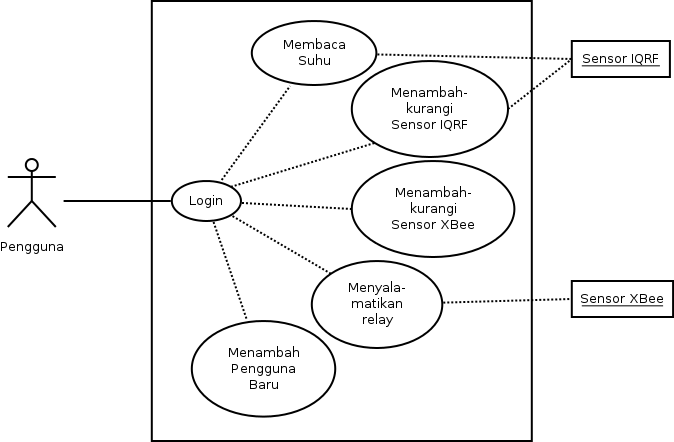
\includegraphics[width=0.9\textwidth]{gambar/usecase}
				    \caption{Diagram \emph{use case} dari penelitian.}
				    \label{usecase}
				\end{figure}

			Pada Gambar \ref{usecase}, menambah-kurangi sensor XBee tidak melibatkan sensor XBee (tidak ada garis yang menghubungkan keduanya), pada \emph{case} tersebut hanya melibatkan aplikasi. Saat \emph{case} ini dijalankan, data sensor pada basis data dihapus. Namun, menambah-kurangi sensor IQRF melibatkan sensor IQRF (ada garis yang menghubungkan keduanya). Karena pada \emph{case} ini, selain menghapus data pada basis data, proses \emph{unbonding} pada IQRF juga melibatkan \emph{node} IQRF.

		\subsection{Diagram Arsitektur Sistem}
			Penelitian ini menggunakan AP, \emph{sensor coordinator}, dan \emph{sensor node} sebagai piranti keras. Sedangkan piranti lunak yang dikembangkan meliputi aplikasi berbasis web, aplikasi Python, dan aplikasi C yang terunggah pada sensor-sensor. Gambar \ref{system-architecture} menggambarkan diagram arsitektur sistem.
			
			\begin{figure}[H]
			  \centering
			    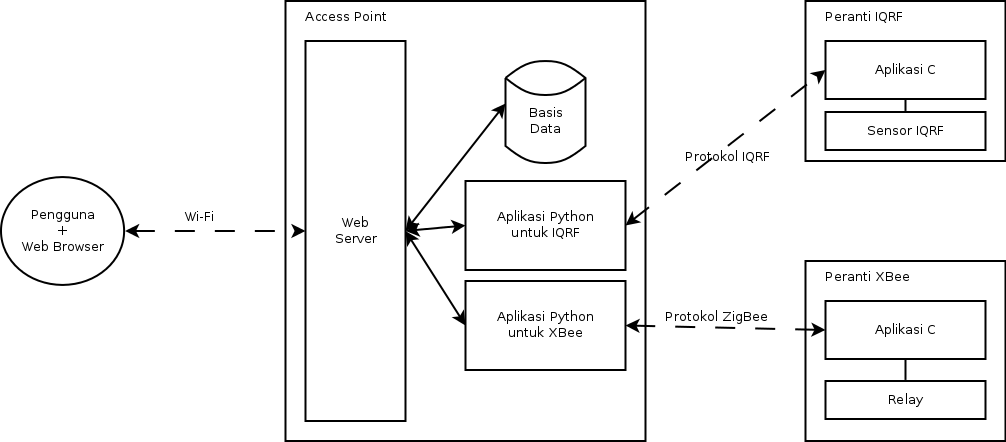
\includegraphics[width=\textwidth]{gambar/system-architecture}
			    \caption{Diagram Arsitektur Sistem.}
			    \label{system-architecture}
			\end{figure}

			Seperti terlihat pada Gambar \ref{system-architecture}, pengguna yang ingin mengakses aplikasi berbasis web guna mengendalikan sensor harus menggunakan web browser. Web browser yang dimaksud tidak terbatas hanya yang terinstal pada komputer, namun juga web browser yang terdapat pada ponsel cerdas atau komputer tablet.

		\subsection{\emph{Software Development Life Cycle} (SDLC)}
			Pengembangan aplikasi ini menggunakan konsep pengembangan iteratif dan inkremental. Pada konsep pengembangan ini, kode-kode aplikasi dirancang, dikembangkan, dan diuji pada siklus yang terulang. Pada tiap iterasi, fitur tambahan dapat dirancang, dikembangkan, dan diuji sampai terbangun aplikasi yang berfungsi seperti yang dikehendaki. Ilustrasi SDLC yang digunakan dapat dilihat pada Gambar \ref{sdlc}.

			\begin{figure}[H]
			  \centering
			    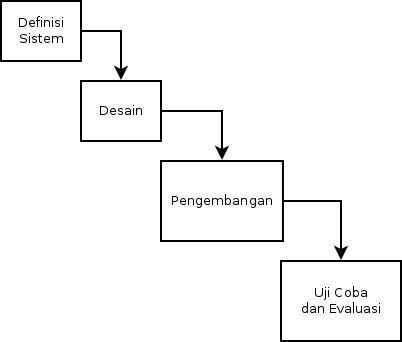
\includegraphics[width=0.6\textwidth]{gambar/sdlc}
			    \caption{Diagram SDLC.}
			    \label{sdlc}
			\end{figure}

			Aplikasi akan dikembangkan fitur demi fitur dan diuji apakah masing-masing fitur dapat berjalan sebagaimana mestinya. Masing-masing aplikasi yang dikembangkan (aplikasi web, Python, dan C) juga akan dikembangkan dan diuji apakah masing-masing aplikasi dapat saling berinteraksi. Iterasi terus dilakukan hingga fitur-fitur dan aplikasi-aplikasi tersebut dapat berfungsi untuk interoperabilitas \emph{Wireless Sensor Network} (WSN) dan protokol Internet.
	
	\section{Pengembangan Aplikasi}
		Tahap-tahap dalam pengembangan aplikasi adalah persiapan, pengembangan aplikasi WSN yang ditulis dengan bahasa C, pengembangan aplikasi Python untuk menghubungkan aplikasi web dan sensor, pengembangan aplikasi berbasis web, serta evaluasi dan perbaikan.

		\subsection{Persiapan Pra Pengembangan Aplikasi}
			Persiapan yang harus dilakukan sebelum mengembangkan aplikasi adalah mengkonfigurasi router/AP, mengkonfigurasi komputer yang akan digunakan untuk pengembangan aplikasi, dan mengkonfigurasi pengalamatan pada XBee.

			
			\subsubsection{Konfigurasi Router/\emph{Access Point} (AP)} \

				Penelitian ini menggunakan AP keluaran TP-LINK seri MR3020. AP jenis ini dipilih karena bentuknya yang kecil sehingga mudah dibawa atau dipindahkan dan kemudahannya untuk dimodifikasi. TP-LINK MR3020 juga terbilang populer di ranah komunitas sistem benam (\emph{embedded device}) sehingga memiliki dukungan yang baik dari pabrikan dan komunitas. 

				Sebelum digunakan, \emph{firmware} bawaan TP-LINK MR3020 harus diganti dengan sistem operasi OpenWRT. Proses penggantian cukup mudah karena hanya memanfaatkan menu \emph{firmware upgrade} dari web admin yang sudah tersedia.	Sistem Operasi OpenWRT yang digunakan adalah Attitude Adjustment versi 12.09 dengan Linux kernel 3.3.8. \emph{Image file} sistem operasi tersebut bisa diunduh secara gratis pada situs \url{www.openwrt.org}.

				Setelah OpenWRT berhasil terinstall, langkah selanjutnya adalah mengimplementasikan \emph{extroot}. \emph{Extroot} adalah fitur dari OpenWRT yang dapat memetakan direktori \emph{root} pada memori eksternal, sehingga \emph{extroot} dapat memperbesar memori penyimpanan dengan bantuan USB \emph{flash drive}. Langkah yang harus dilakukan pertamakali adalah menginstall perangkat lunak dengan perintah sebagai berikut:
				\begingroup
				    \fontsize{10pt}{12pt}\selectfont
				    \begin{verbatim}
						# opkg update
						# opkg install block-extroot block-hotplug block-mount
				    \end{verbatim}  
				\endgroup

				Kemudian dilanjutkan dengan menyalin isi dari memori internal TP-LINK MR3020 ke USB \emph{flash drive} yang di-\emph{mount} pada direktori /mnt/sda1 dengan perintah:
				\begingroup
				    \fontsize{10pt}{12pt}\selectfont
				    \begin{verbatim}
						# tar -C /overlay -cvf - . | tar -C /mnt/sda1 -xf -
				    \end{verbatim}  
				\endgroup

				Langkah terakhir adalah mengkonfigurasi file /etc/config/fstab dan menyalakan ulang AP. Konfigurasi diganti dengan detil sebagai berikut:
				\begingroup
				    \fontsize{10pt}{12pt}\selectfont
				    \begin{verbatim}
						config mount
					        option target        /mnt
					        option device        /dev/sda1
					        option fstype        ext3
					        option options       rw,sync
					        option enabled       1
					        option enabled_fsck  0
					        option is_rootfs     1
				    \end{verbatim}  
				\endgroup

				Konfigurasi di atas akan memetakan direktori \emph{root} (/) ke dalam piranti (\emph{device}) /dev/sda1 yang di-\emph{mount} pada direktori /mnt dengan format \emph{filesystem} ext3 dan dan mode baca tulis.

				Setelah proses implementasi extroot selesai, berarti AP sudah memiliki memori penyimpanan yang cukup (atau mungkin lebih) untuk menginstal aplikasi-aplikasi pendukung lainnya. Penelitian ini menggunakan memori USB 4 Gigabyte.

				Agar TP-LINK MR3020 dapat membaca dan mengirimkan data dari dan ke WSN melalui kanal serial, dibutuhkan Python dan pustaka PySerial yang diinstal dengan perintah:
				\begingroup
				    \fontsize{10pt}{12pt}\selectfont
				    \begin{verbatim}
						# opkg update
						# opkg install python pyserial
				    \end{verbatim}  
				\endgroup

				Sedangkan paket aplikasi `at' digunakan agar AP dapat menjalankan perintah untuk menyala-matikan relay pada waktu tertentu. Namun, sebelum at dapat berjalan, pada router sudah harus tersedia file /var/spool/cron/atjobs/.SEQ dan pemilik dari file tersebut harus diganti menjadi daemon.daemon. Aplikasi `at' diinstall dengan perintah:
				\begingroup
				    \fontsize{10pt}{12pt}\selectfont
				    \begin{verbatim}
						# opkg update && opkg install at
				    \end{verbatim}  
				\endgroup
				
				Langkah selanjutnya adalah instalasi aplikasi pendukung aplikasi berbasis web yang nantinya akan dikembangkan yaitu Web Server, PHP, dan MySQL. Web server yang digunakan adalah yang sudah terinstal pada OpenWRT versi Attitude Adjustment yaitu uHTTPd. Sedangkan PHP dan MySQL harus diinstal dengan perintah:
				\begingroup
				    \fontsize{10pt}{12pt}\selectfont
				    \begin{verbatim}
						# opkg update
						# opkg install php5 php5-cgi mysql
				    \end{verbatim}  
				\endgroup

				Setelah PHP berhasil terinstal, buka file /etc/config/uhttpd dan pastikan baris yang memuat baris di bawah ini tidak dalam keadaan terkomentar.

				\begingroup
				    \fontsize{10pt}{12pt}\selectfont
				    \centering
				    \begin{verbatim}
						list interpreter ".php=/usr/bin/php-cgi"
				    \end{verbatim}  
				\endgroup					

				Aplikasi yang terakhir yang harus diinstal adalah SSHFS yang berguna dalam uji coba dan perbaikan aplikasi. SSHFS dapat diinstal dengan perintah:
				\begingroup
				    \fontsize{10pt}{12pt}\selectfont
				    \begin{verbatim}
						# opkg update
						# opkg install sshfs
				    \end{verbatim}  
				\endgroup

				Zona waktu standar pada OpenWRT adalah UTC yang berlokasi pada kota Greenwich di Inggris Raya. Agar zona waktu dapat dikonfigurasi sesuai dengan zona waktu kota Yogyakarta, maka isi dari file /etc/config/system harus disesuaikan. Pada file tersebut, zona waktu UTC diganti menjadi WIT-7 atau \emph{Western Indonesian Time}-7.

			\subsubsection{Konfigurasi Komputer untuk Pengembangan} \

				Komputer yang digunakan dalam penelitian ini adalah MacBook Pro dengan sistem operasi Mac OS X Mountain Lion. Sedangkan aplikasi yang harus tersedia adalah Sublime Text 3, Arduino for Mac OS X, CoolTerm, Driver FTDI for Mac OS X, IQRF IDE v 2.08 for TR-53B.

				Sublime Text 3 berperan banyak dalam mengedit kode-kode sumber PHP, C, dan Python.

				Sedangkan proses pengembangan dan pengunduhan aplikasi untuk Arduino sepenuhnya dilakukan dengan Arduino for Mac OS X karena aplikasi tersebut sudah mencakup editor teks dan alat kompilasi.

				Agar komputer dapat membaca kanal serial sehingga dapat melakukan tugas-tugas seperti konfigurasi XBee Radio dan pengujian aplikasi Python, komputer membutuhkan aplikasi CoolTerm. Sebelum aplikasi ini terinstal, pastikan \emph{driver} FTDI untuk Mac OS X sudah terinstal, agar komputer dapat mendeteksi XBee yang terhubung melalui USB.

				Walaupun kode sumber untuk IQRF ditulis dengan bantuan Sublime Text 3, proses kompilasinya dilakukan dengan aplikasi IQRF IDE v 2.08 for TR-53B. Proses pengunduhan file ke IQRF juga dilakukan dengan aplikasi yang sama.

				Semua proses instalasi aplikasi yang dibutuhkan dilakukan dengan prosedur standar dari Mac OS X. Yaitu memperoleh file binary-nya dan kemudian menyalin file tersebut ke direktori Application atau mengikuti prosedur standar dari masing-masing aplikasi.

				Langkah terakhir yang dilakukan adalah memastikan AP dapat mengakses komputer melalui SSH. Pastikan \emph{remote sharing} dalam keadaan tercentang di \emph{System Preference}, \emph{Sharing}. Atau untuk lebih jelasnya dapat melihat pada Gambar \ref{mac-sharing}.

				\begin{figure}[H]
				  \centering
				    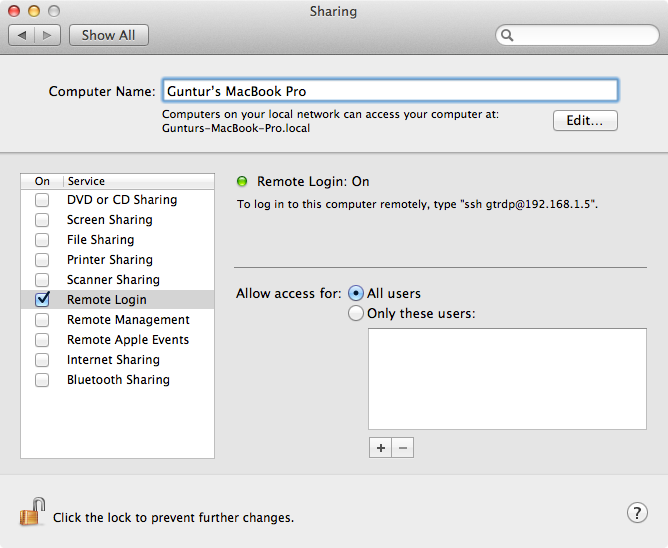
\includegraphics[width=0.8\textwidth]{gambar/mac-sharing}
				    \caption{Konfigurasi SSH pada Mac OS X.}
				    \label{mac-sharing}
				\end{figure}

			\subsubsection{Piranti XBee}\

				Setiap piranti XBee yang akan digunakan harus terkonfigurasi terlebih dahulu. Parameter-parameter yang harus terkonfigurasi adalah ATID (alamat dari jaringan/\emph{network ID}), ATMY (alamat piranti itu sendiri), ATDH (\emph{destination address high}), dan ATDL (\emph{destination address low}).

				Proses konfigurasi dilakukan dengan menyambungkan XBee Radio dengan \emph{XBee Explorer USB Board} ke komputer dan menjalankan aplikasi untuk membaca kanal serial, misalnya CoolTerm pada Mac OS X. Setelah CoolTerm dibuka, buka koneksi kanal serial ke XBee dan jalankan perintah dengan format:
				\begingroup
				    \fontsize{10pt}{12pt}\selectfont
				    \begin{verbatim}
						+++		#masuk ke AT Mode
						ATID <id jaringan>
						ATMY <alamat dari zigbee>
						ATDH <destination high>
						ATDL <destination low>
						ATWR 	#tulis ke non volatile memory
				    \end{verbatim}  
				\endgroup

				Contoh perintahnya adalah:
				\begingroup
				    \fontsize{10pt}{12pt}\selectfont
				    \begin{verbatim}
						+++		#masuk ke AT Mode
						ATID 1234
						ATMY 5
						ATDH 0
						ATDL 1
						ATWR 	#tulis ke non volatile memory
				    \end{verbatim}  
				\endgroup

		\subsection{Pengembangan Aplikasi WSN}
			Langkah selanjutnya yang dilakukan dalam pengembangan adalah pengembangan aplikasi untuk WSN yang terdiri atas aplikasi C yang masing-masing ditujukan untuk IQRF dan XBee. Setelah aplikasi selesai ditulis, kode sumber kemudian di-\emph{compile} dan diunduh ke dalam WSN.

			\subsubsection{Aplikasi IQRF}\

				Piranti IQRF dalam penelitian ini ada dua jenis, begitu pula aplikasi yang tertanam di dalamnya. Aplikasi tersebut adalah \emph{Sink} dan \emph{Node}. Aplikasi \emph{Sink} akan ditanamkan pada koordinator dari IQRF yang terhubung langsung dengan AP melalui kabel USB dan jumlahnya hanya satu. Sedangkan aplikasi \emph{Node} akan ditanamkan pada sensor-sensor IQRF yang akan saling membentuk jaringan jala (\emph{mesh network}) dan jumlahnya lebih dari satu.

				Aplikasi \emph{Sink} lebih ditekankan pada pembentukan ikatan (\emph{bond}) antara koordinator dan sensor-sensor, pengendalian sensor-sensor, serta pengakuisisian data dari masing-masing sensor.

				Sedangkan aplikasi \emph{Node} lebih bersifat pasif karena hanya akan merespon perintah-perintah yang akan dikirimkan oleh koordinator, seperti pembentukan ikatan dan pembacaan temperatur.

				Data yang akan diakuisisi dari masing-masing sensor adalah temperatur yang terbaca di masing-masing sensor.

				Aplikasi yang digunakan adalah aplikasi iHome yang dikembangkan oleh \cite{widyawan2012ihome} yang fiturnya sebenarnya tidak terbatas hanya pada pembacaan temperatur sekitar.

			\subsubsection{Aplikasi XBee}\

				Sama seperti IQRF, piranti XBee terdiri dari dua jenis piranti, yaitu koordinator dan sensor-sensor. Koordinator bertugas menyalakan atau mematikan relay-relay yang terdapat di masing-masing sensor sesuai permintaan pengguna.

				Koordinator tersusun atas \emph{XBee 802.15.4 Radios (Series 1)} yang tertanam pada \emph{XBee Explorer USB Board} dan terkoneksi langsung dengan AP dengan kabel USB.

				Sedangkan sensornya terdiri dari tiga bagian, yaitu \emph{XBee 802.15.4 Radios (Series 1)}, \emph{2 channel Relay Shield For Arduino (With XBee/BTBee interface)}, dan Arduino Uno. Ketiga bagian tersebut saling terhubung dengan pin-pin yang tersedia.

				XBee pada hakikatnya hanya sebatas piranti komunikasi antara AP dengan relay-relay yang tersedia, sehingga pemrograman teletak pada masing-masing Arduino pada relay. Bahasa yang digunakan adalah bahasa C (Arduino). Aplikasi yang dikembangkan akan menunggu perintah dari AP untuk menyalakan atau mematikan relay.

		\subsection{Pengembangan Aplikasi Python}
			Aplikasi Python adalah jantung dari penelitian ini karena menghubungkan aplikasi berbasis web dengan piranti-piranti IQRF dan XBee.	Aplikasi terdiri dari tiga bagian yang ditujukan untuk penggunaan berbeda, yaitu komunikasi dengan sensor IQRF, XBee, dan profil untuk automatisasi.

			\subsubsection{Manipulasi Komunikasi Data Serial}\

				Aplikasi yang nantinya tertanam pada AP, yaitu aplikasi berbasis web dan aplikasi Python, akan berjalan di atas sistem operasi OpenWrt. Hal ini berarti aplikasi yang dibangun tidak akan bersentuhan secara langsung dengan aliran data aras rendah seperti aliran bit-bit data. Segala bentuk komunikasi data aras rendah yang melibatkan bit-bit data dikelolah sepenuhnya oleh OpenWrt sehingga aras terendah dari komunikasi data yang terbaca oleh aplikasi adalah pada aras karakter yang saling dipertukarkan oleh masing-masing aplikasi yang dibangun. Hal ini dijelaskan dengan ilustrasi sebagai berikut.

				\begin{figure}[H]
				  \centering
				    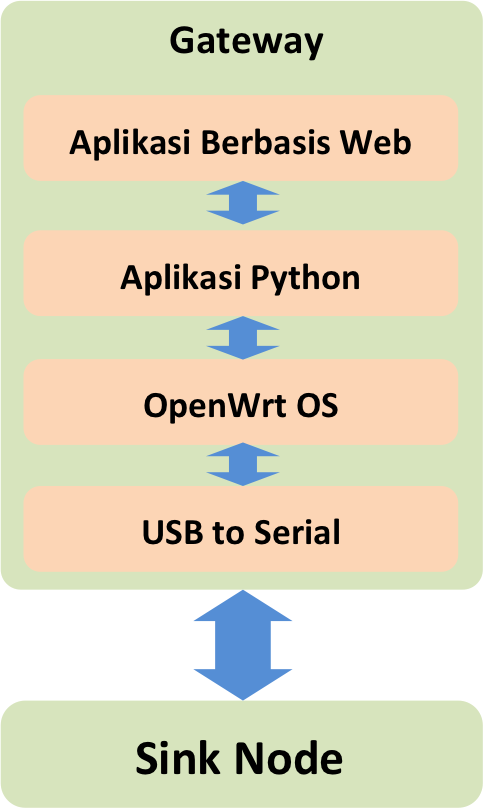
\includegraphics[width=0.4\textwidth]{gambar/manipulation}
				    \caption{Manipulasi komunikasi data serial \cite{wibowo2013wireless}.}
				    \label{manipulation}
				\end{figure}

				Dari Gambar \ref{manipulation}, tampak bahwa alur manipulasi data serial aras rendah dari \emph{sink node} dimulai dari USB to serial, sistem operasi OpenWrt, aplikasi Python, kemudian pada akhirnya aplikasi berbasis web. Pengubahan bit-bit data serial terjadi pada bagian OpenWrt OS.

			\subsubsection{Aplikasi IQRF}\

				Aplikasi Python IQRF memiliki kemampuan untuk melakukan \emph{bonding} antara koordinator dan sensor, dan pembacaan temperatur pada sensor dengan ID tertentu.

				Diagram alir dari aplikasi berikut dapat dilihat pada Gambar \ref{python-iqrf}.

				\begin{figure}[H]
				  \centering
				    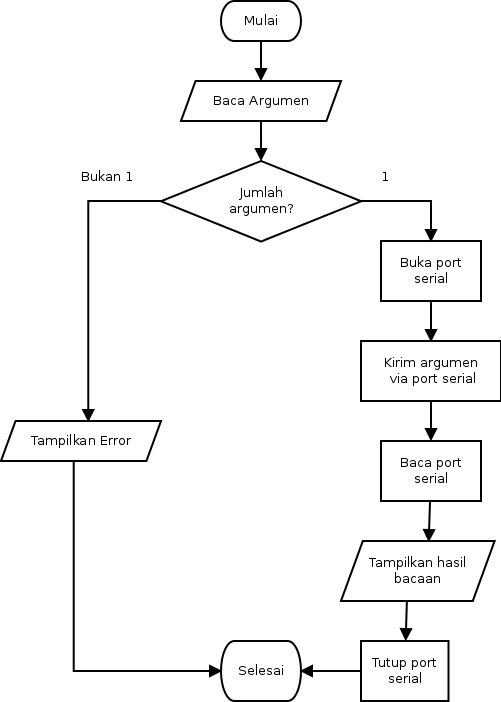
\includegraphics[width=0.6\textwidth]{gambar/python-iqrf}
				    \caption{Diagram alir aplikasi Python untuk IQRF.}
				    \label{python-iqrf}
				\end{figure}

				Aplikasi dijalankan dengan menjalankan format perintah berikut pada \emph{terminal console}:
				\begingroup
				    \fontsize{10pt}{12pt}\selectfont
				    \begin{verbatim}
						$ python iqrf.py <perintah><ID node>
				    \end{verbatim}  
				\endgroup

				Aplikasi ini berjalan dalam bentuk CLI dan membutuhkan satu parameter, yaitu perintah yang langsung disambung dengan ID node tanpa spasi. Perintah yang tersedia yaitu membaca gemperatur pada node ID tertentu (g), \emph{bonding} node ID tertentu (b), \emph{unbonding} node ID tertentu (u).

				Sehingga contoh penggunaan aplikasi pada \emph{terminal console}:
				\begingroup
				    \fontsize{10pt}{12pt}\selectfont
				    \begin{verbatim}
						$ python iqrf.py g3
				    \end{verbatim}  
				\endgroup
				Perintah di atas adalah perintah untuk membaca temperatur pada node ID 3.

			\subsubsection{Aplikasi XBee}\

				Aplikasi Python XBee memiliki kemampuan untuk menyalakan atau mematikan relay pada piranti tertentu dan membaca status relay pada piranti tertentu, apakah relay tersebut sedang menyala atau mati.

				Diagram alir dari aplikasi berikut dapat dilihat pada Gambar \ref{python-xbee}.

				\begin{figure}[H]
				  \centering
				    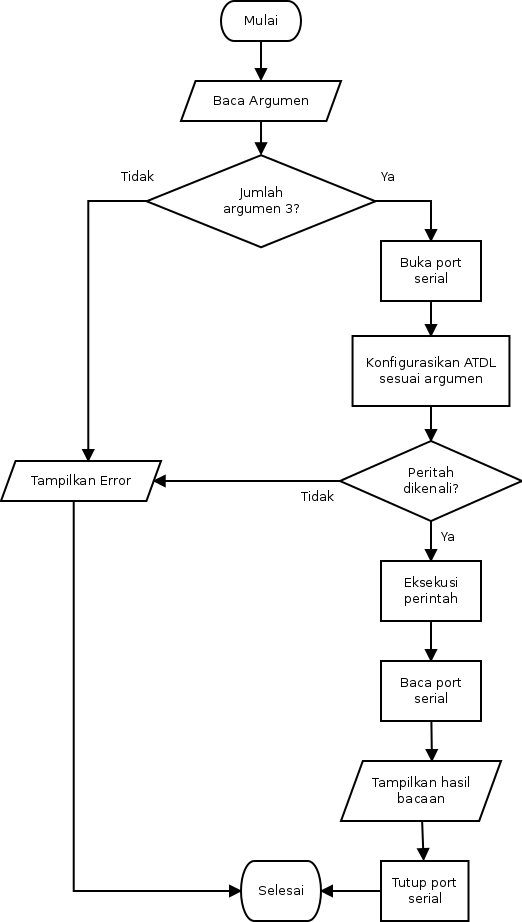
\includegraphics[width=0.6\textwidth]{gambar/python-xbee}
				    \caption{Diagram alir aplikasi Python untuk menangani piranti XBee.}
				    \label{python-xbee}
				\end{figure}

				Aplikasi dijalankan dengan menjalankan format perintah berikut pada \emph{terminal console}:
				\begingroup
				    \fontsize{10pt}{12pt}\selectfont
				    \begin{verbatim}
						$ python xbee.py <perintah> <ATMY piranti> <ID relay>
				    \end{verbatim}  
				\endgroup

				Aplikasi ini berjalan dalam bentuk CLI dan membutuhkan tiga parameter, yaitu perintah, alamat piranti (ATMY), dan ID relay (terdapat dua relay di tiap piranti). Perintah yang tersedia yaitu menyalakan relay, `on', mematikan relay, `off', dan membaca status relay, `status'.

				Sehingga contoh penggunaan aplikasi pada \emph{terminal console}:
				\begingroup
				    \fontsize{10pt}{12pt}\selectfont
				    \begin{verbatim}
						$ python iqrf.py status 2 1
				    \end{verbatim}  
				\endgroup
				Perintah di atas akan membaca status (on/off) dari relay 1 pada piranti dengan alamat (ATMY) 2 dan menampilkannya pada layar dalam karakter `H' (menyala) atau `L' (mati).

			\subsubsection{\emph{Profiling}}\

				Aplikasi ini memanfaatkan aplikasi \emph{at} pada Linux yang dapat menjalankan perintah tertentu di \emph{terminal console} pada waktu tertentu. Dengan aplikasi ini, pengguna dapat menyala-matikan relay pada waktu tertentu. Jika hal ini dikombinasikan dengan bacaan temperatur dari sensor IQRF, maka pengguna dapat menyala-matikan relay tertentu pada saat temperatur pada sensor IQRF node tertentu mencapai suhu tertentu, dan juga bisa hanya terjadi saat waktu tertentu.

				Diagram alir dari aplikasi berikut dapat dilihat pada Gambar \ref{python-profile}.

				\begin{figure}[H]
				  \centering
				    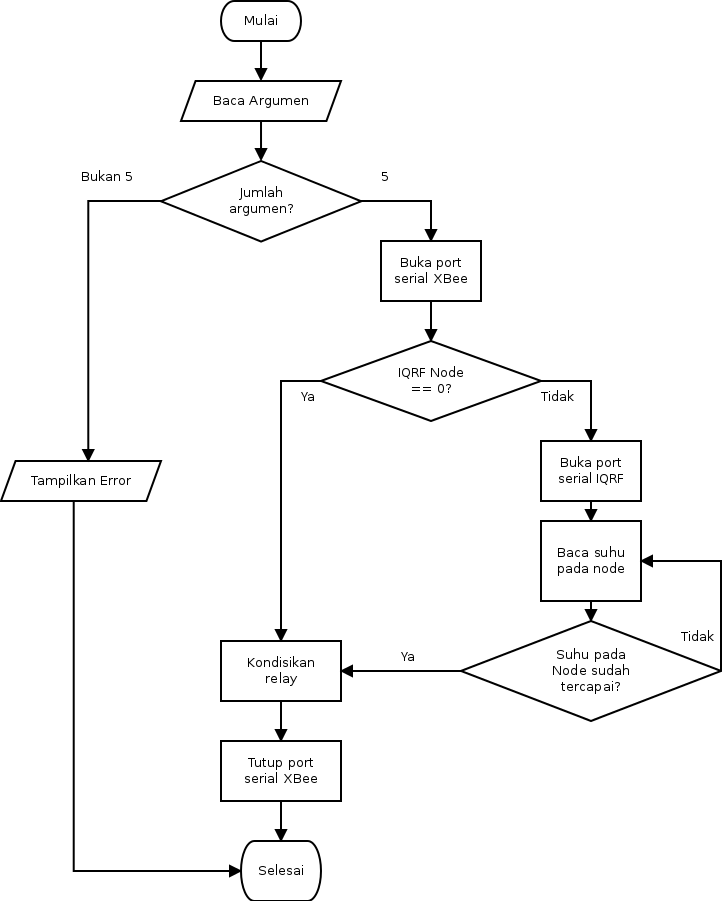
\includegraphics[width=0.8\textwidth]{gambar/python-profile}
				    \caption{Diagram alir aplikasi Python untuk menyala-matikan lampu pada kondisi tertentu.}
				    \label{python-profile}
				\end{figure}


		\subsection{Pengembangan Aplikasi Berbasis Web}
			Aplikasi web untuk mengendalikan sensor-sensor IQRF dan XBee dibangun dengan PHP dan basis data MySQL. Aplikasi ini dibangun tanpa menggunakan \emph{framework} karena aplikasi ini tergolong tidak terlalu rumit, aplikasi ini hanya memliki lima halaman utama seperti terlihat pada sitemap Gambar \ref{sitemap}. Penggunaan \emph{framework} juga akan memakan sumber daya komputasi sedikit lebih banyak, padahal aplikasi ini akan diimplementasikan pada sebuah AP yang memiliki tingkat komputasi yang rendah.

			Antarmuka yang dikembangkan adalah hasil \emph{fork} dari \emph{template} halaman administrator buatan Vince G \cite{Gabriel2013}. Antarmuka ditulis menggunakan HTML5 dan CSS3, dengan tambahan pemrograman JavaScript pada sisi klien agar menambah interaktivitas. Pustaka Bootstrap digunakan untuk membuat halaman web menjadi responsif, sehingga dapat menyesuaikan diri secara otomatis sesuai dengan ukuran layar. Pustaka jQuery digunakan untuk membantu pemrograman di sisi klien.

			Kode sumber untuk aplikasi berbasis web ditulis dengan bantuan Sublime Text 3.
			
			Peta situs dari aplikasi berbasis web yang dikembangkan dapat dilihat pada Gambar \ref{sitemap}.
			
			\begin{figure}[H]
			  \centering
			    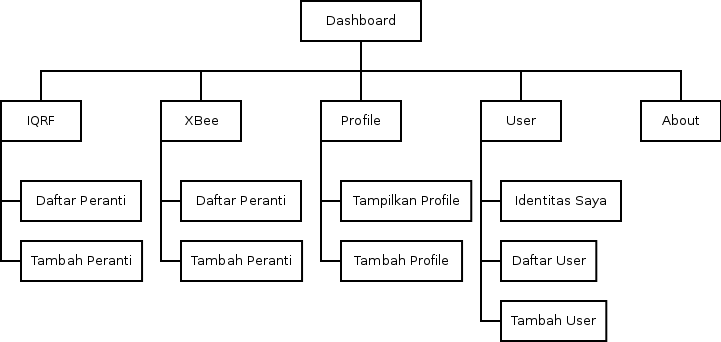
\includegraphics[width=0.8\textwidth]{gambar/sitemap}
			    \caption{Peta situs aplikasi web.}
			    \label{sitemap}
			\end{figure}

			Total halaman utama dari situs ada enam halaman, seperti dapat dilihat pada Gambar \ref{sitemap} dengan tambahan halaman login, halaman yang harus diakses sebelum pengguna dapat masuk ke dalam sistem. Empat halaman utama mempunyai halaman anak yang secara garis besar ditujukan untuk melihat, menghapus dan menambah piranti, profil, atau pengguna.

			Basis data yang dikembangkan tergolong sederhana karena hanya dimaksudkan untuk menyimpan data-data yang sifatnya kecil, seperti tampak pada Gambar \ref{erd}.

			\begin{figure}[H]
			  \centering
			    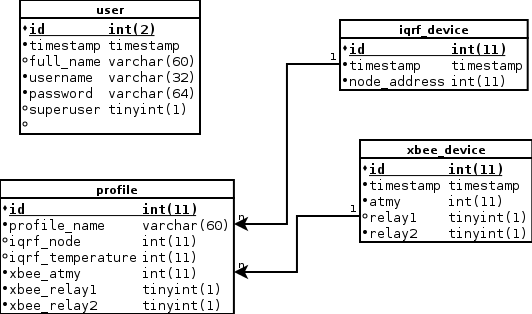
\includegraphics[width=0.6\textwidth]{gambar/erd}
			    \caption{\emph{Entity Relationship Diagram} dari basis data untuk aplikasi web.}
			    \label{erd}
			\end{figure}

			Seperti yang terpampang pada Gambar \ref{erd}, basis data terdiri atas empat tabel. Relasi yang ada pada basis data hanya relasi tabel \emph{iqrf\_device} dengan \emph{profile} dan \emph{xbee\_device} dengan \emph{profile}.

			Sedangkan diagram alir untuk menambah piranti IQRF dan XBee dijelaskan pada Gambar \ref{add-iqrf} dan Gambar \ref{add-xbee}.

			\begin{figure}[H]
			  \centering
			    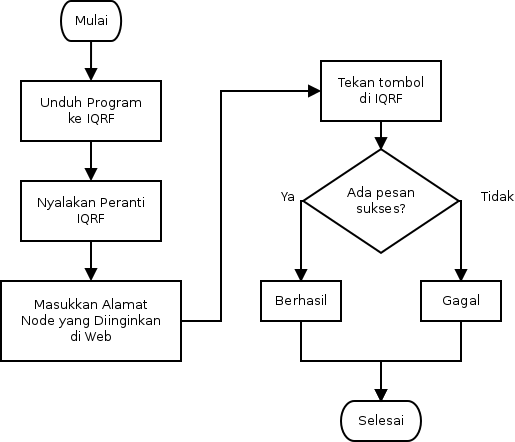
\includegraphics[width=0.6\textwidth]{gambar/add-iqrf}
			    \caption{Diagram Alir Penambahan Piranti IQRF ke Aplikasi.}
			    \label{add-iqrf}
			\end{figure}

			\begin{figure}[H]
			  \centering
			    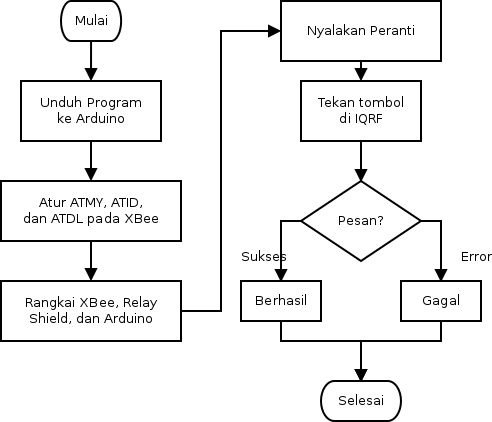
\includegraphics[width=0.6\textwidth]{gambar/add-xbee}
			    \caption{Diagram Alir Penambahan Piranti XBee ke Aplikasi.}
			    \label{add-xbee}
			\end{figure}

			Penambahan piranti IQRF mengharuskan pengguna untuk menekan tombol yang ada pada sensor IQRF, sedangkan penambahan piranti XBee tidak mengharuskan pengguna untuk menekan tombol atau mengintervensi perangkat keras XBee.

		\subsection{Skalabilitas Sistem}
			Seperti yang sudah dijelaskan sebelumnya tentang rancangan teknis sistem, secara \emph{default} aplikasi ini hanya mendukung interoperabilitas antara dua jenis WSN. Karena pendekatan interoperabilitas dilakukan pada ranah data dan aplikasi disusun hanya untuk mendukun dua jenis WSN, sistem tidak memiliki skalabilitas dalam hal penambahan jenis WSN. Jika diinginkan jenis WSN baru yang ingin diinteroperabilitaskan, maka harus ditambahkan beberapa baris kode baru untuk menangani WSN baru yang mungkin struktur komunikasinya sedikit berbeda.

			Walaupun demikian, sistem yang dibangun memiliki skalabilitas dalam hal penambahan jumlah piranti yang terpasang. Piranti atau \emph{node} yang ingin dipantau dengan aplikasi dapat ditambahkan dan dikurangi melalui antarmuka yang telah dirancang dengam mudah.


		\subsection{Evaluasi dan Perbaikan}
			Evaluasi dilakukan dengan mengujikan semua fitur yang dimiliki oleh aplikasi. Jika terdapat kesalahan, maka dilacak dimanakah letak kesalahan berada, apakah pada aplikasi berbasis web, aplikasi Python, atau aplikasi C pada sensor.

			Masalah yang timbul adalah saat akan merevisi aplikasi yang sudah terlanjur tertanam pada AP karena AP, dengan sistem operasi OpenWRT, tidak memiliki aplikasi teks editor yang mumpuni untuk melakukan pengeditan kode sumber dengan nyaman. Oleh karena itu, seluruh kode sumber tetap berada pada komputer agar tetap bisa dibuka dengan Sublime Text 3, namun AP me-\emph{mount}-nya dengan bantuan SSHFS sehingga seolah-olah kode sumber tersebut berada dalam dua tempat dan saling tersinkronisasi.

			\emph{Mounting} pada AP dilakukan dengan menggunakan perintah:
			\begingroup
			    \fontsize{10pt}{12pt}\selectfont
			    \begin{verbatim}
					# sshfs /direktori/pada/ap <user>@<alamat IP>:/direktori/pada/komputer
			    \end{verbatim}  
			\endgroup

			Contoh penggunaan perintah tersebut:
			\begingroup
			    \fontsize{10pt}{12pt}\selectfont
			    \begin{verbatim}
					# sshfs /www/web/ gtrdp@192.168.1.1:/var/www/web/
			    \end{verbatim}  
			\endgroup
			

		\subsection{\emph{Screenshot} Aplikasi}
			Bagian ini menampilkan beberapa \emph{screenshot} dari aplikasi web yang dikembangkan.

			Halaman pertama yang akan terbuka setelah pengguna melakukan \emph{log in} adalah halaman \emph{dashboard} seperti yang dapat dilihat pada Gambar \ref{dashboard}. Tampilan halaman web akan menyesuaikan dengan layar pengguna karena halaman tersebut didesain responsif.

				\begin{figure}[H]
					\begin{subfigure}[b]{\textwidth}
						\centering
					    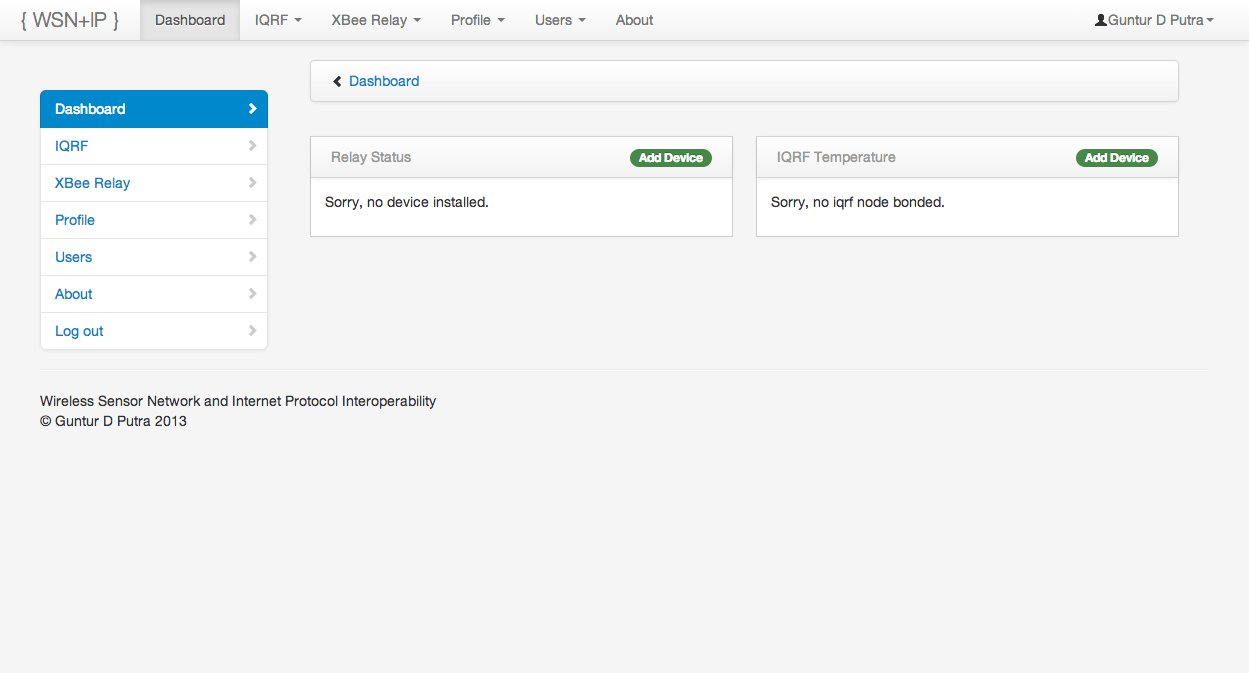
\includegraphics[width=0.9\textwidth]{gambar/dashboard}
					    \caption{Dibuka pada layar komputer.}
					    \label{dashboard-full-page}
					\end{subfigure}
					 ~
					\begin{subfigure}[b]{\textwidth}
						\centering
					    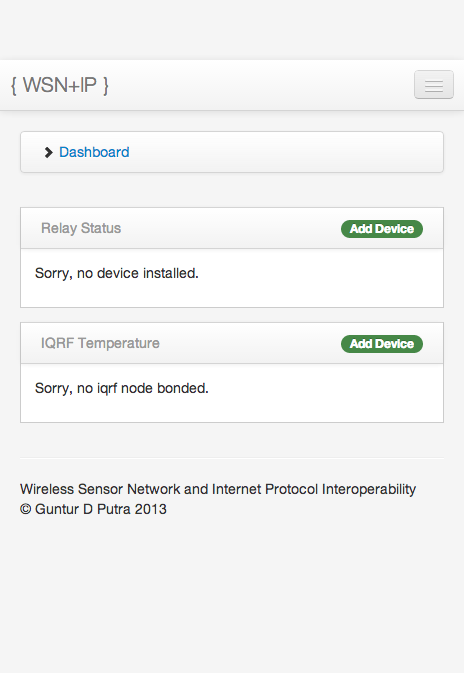
\includegraphics[width=0.3\textwidth]{gambar/dashboard-small}
					    \caption{Dibuka di layar ponsel yang kecil.}
					    \label{dashboard-small}
					\end{subfigure}
					\caption{Halaman \emph{dashboard} saat belum ada piranti terpasang.}
					\label{dashboard}
				\end{figure}

			Seperti dapat dilihat pada Gambar \ref{dashboard-small}, ukuran layar akan menjadi lebih kecil jika dibanding dengan Gambar \ref{dashboard-full-page} karena halaman dibuka pada ponsel cerdas yang memiliki ukuran layar lebih kecil dari komputer.

			Aplikasi mempunyai halaman untuk menambahkan piranti IQRF, sehingga pengguna dapat menambahkan piranti IQRF baru ke dalam sistem menggunakan halaman ini. Gambar \ref{iqrf-add} menunjukkan halaman untuk menambahkan piranti IQRF.

				\begin{figure}[H]
				  \centering
				    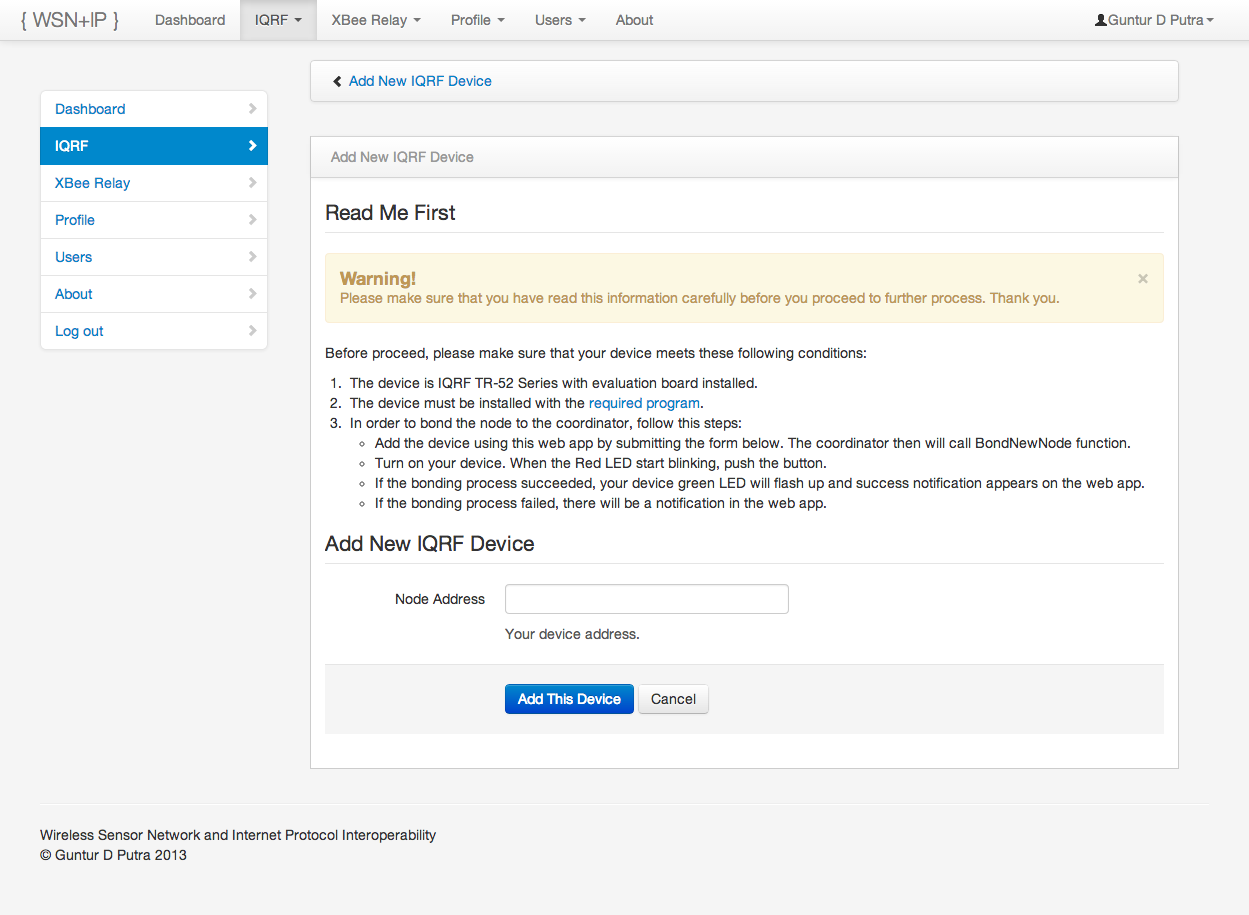
\includegraphics[width=0.9\textwidth]{gambar/iqrf-add}
				    \caption{Halaman untuk menambahkan piranti IQRF.}
				    \label{iqrf-add}
				\end{figure}

			Seperti dapat dilihat pada Gambar \ref{iqrf-add}, pengguna diharuskan untuk memasukkan alamat \emph{node} dari IQRF yang akan ditambahkan. Alamat tersebut adalah bilangan bulat dari dua dan tidak boleh menggunakan alamat yang sudah terpasang pada sistem. Pada bagian atas halaman, terdapat langkah-langkah yang harus diikuti pengguna untuk menambahkan piranti IQRF baru.

			Seperti piranti IQRF, aplikasi juga menyediakan halaman khusus untuk menambahkan piranti XBee, seperti yang dapat dilihat pada Gambar \ref{xbee-add}.

				\begin{figure}[H]
				  \centering
				    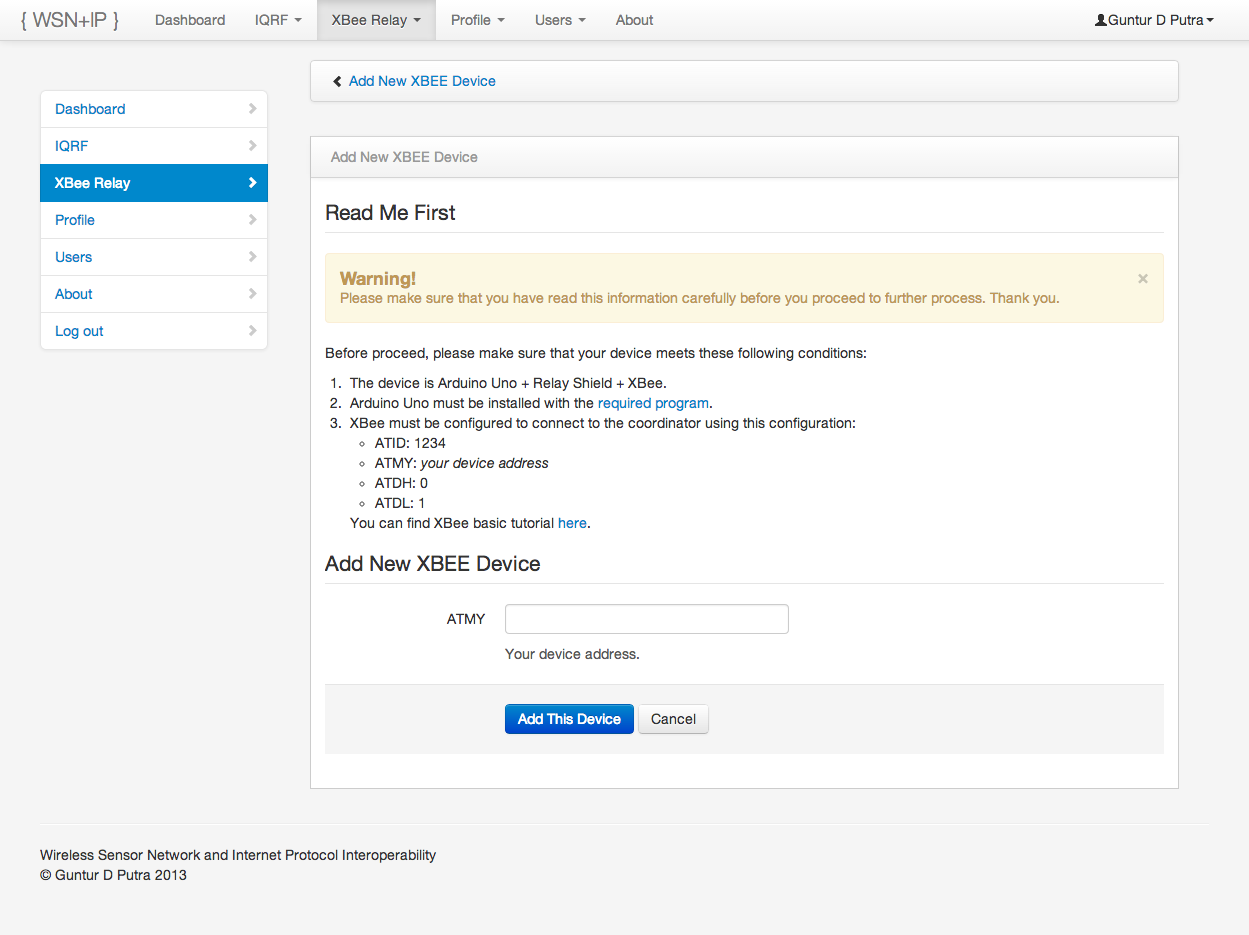
\includegraphics[width=0.9\textwidth]{gambar/xbee-add}
				    \caption{Halaman untuk menambahkan piranti XBee.}
				    \label{xbee-add}
				\end{figure}

			Pengguna juga diharuskan untuk memasukkan alamat ATMY dari XBee yang akan ditambahkan, seperti cara menambahkan piranti IQRF. Pada bagian atas halaman, terdapat langkah-langkah yang harus diikuti pengguna untuk menambahkan piranti XBee baru.

			Saat piranti sudah ditambahkan melalui halaman-halaman yang sudah dijelaskan sebelumnya, halaman \emph{dashboard} akan berubah, seperti yang tergambar pada Gambar \ref{dashboard-full-device}. Halaman ini masih bersifat responsif, sehingga akan menyesuaikan dengan layar di mana halaman tertampil.

				\begin{figure}[H]
				  \begin{subfigure}[b]{\textwidth}
				  \centering
				    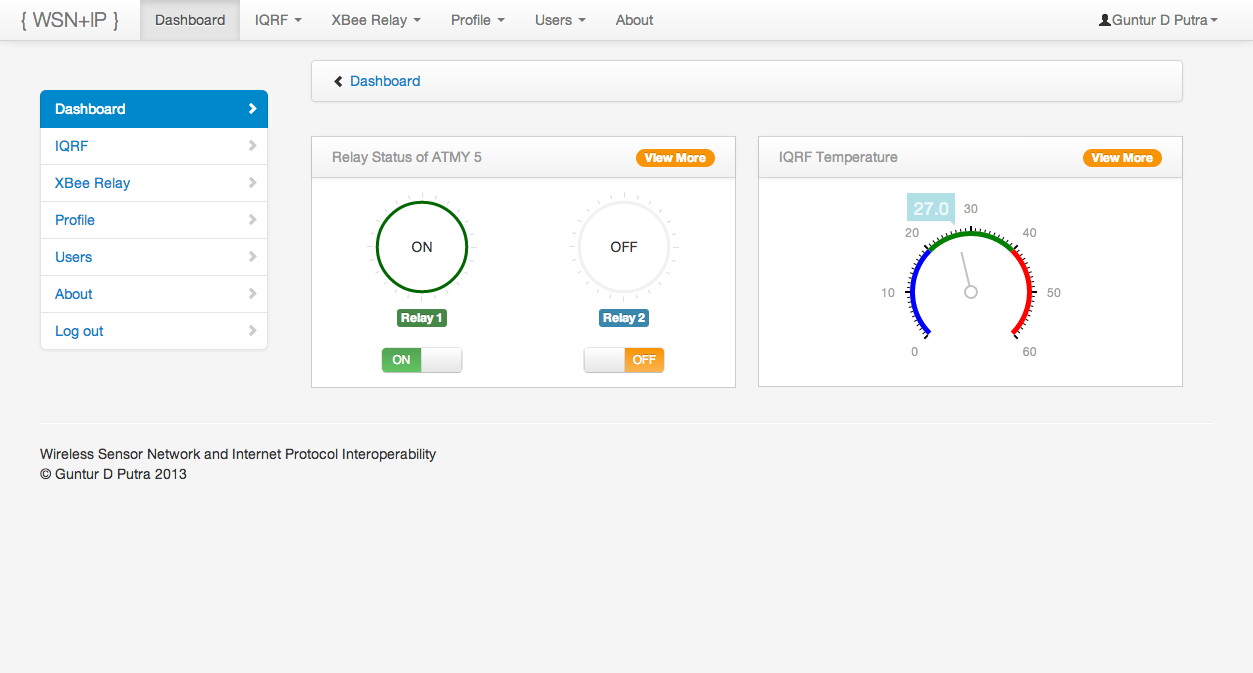
\includegraphics[width=0.9\textwidth]{gambar/dashboard-full}
				    \caption{Dibuka pada layar komputer.}
				    \label{dashboard-full}
				  \end{subfigure}
				~
				  \begin{subfigure}[b]{\textwidth}
				  \centering
				    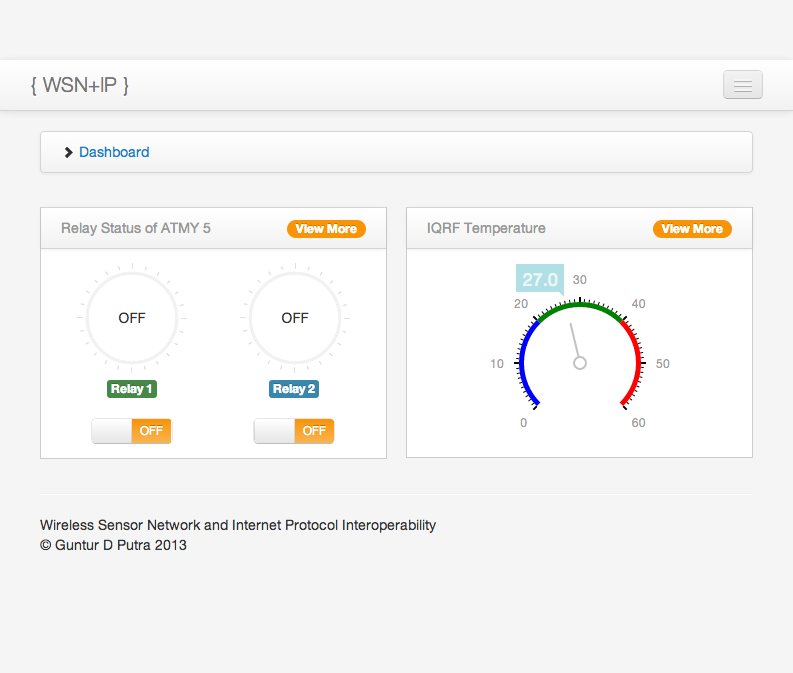
\includegraphics[width=0.6\textwidth]{gambar/dashboard-full-small}
				    \caption{Dibuka pada layar ponsel yang kecil.}
				    \label{dashboard-full-small}
				  \end{subfigure}
				  \caption{Halaman \emph{dashboard} saat piranti sudah terpasang.}
				  \label{dashboard-full-device}
				\end{figure}

			Pada saat halaman dibuka pada layar yang kecil, maka perbedaan yang signifikan adalah hilangnya \emph{sidebar} dan mengecilnya \emph{navigation bar} seperti yang dapat dilihat pada Gambar \ref{dashboard-full} dan \ref{dashboard-full-small}.

			Berapapun banyaknya sensor IQRF atau XBee yang terpasang, halaman \emph{dashboard} tetap akan menampilkan satu piranti saja, yaitu piranti yang pertama kali terpasang. Jika penggune ingin melihat semua sensor yang terpasang, pengguna dapat membuka halaman khusus untuk melihat semua sensor IQRF yang terpasang, seperti yang ditunjukkan pada Gambar \ref{iqrf-list}.

				\begin{figure}[H]
				  \centering
				    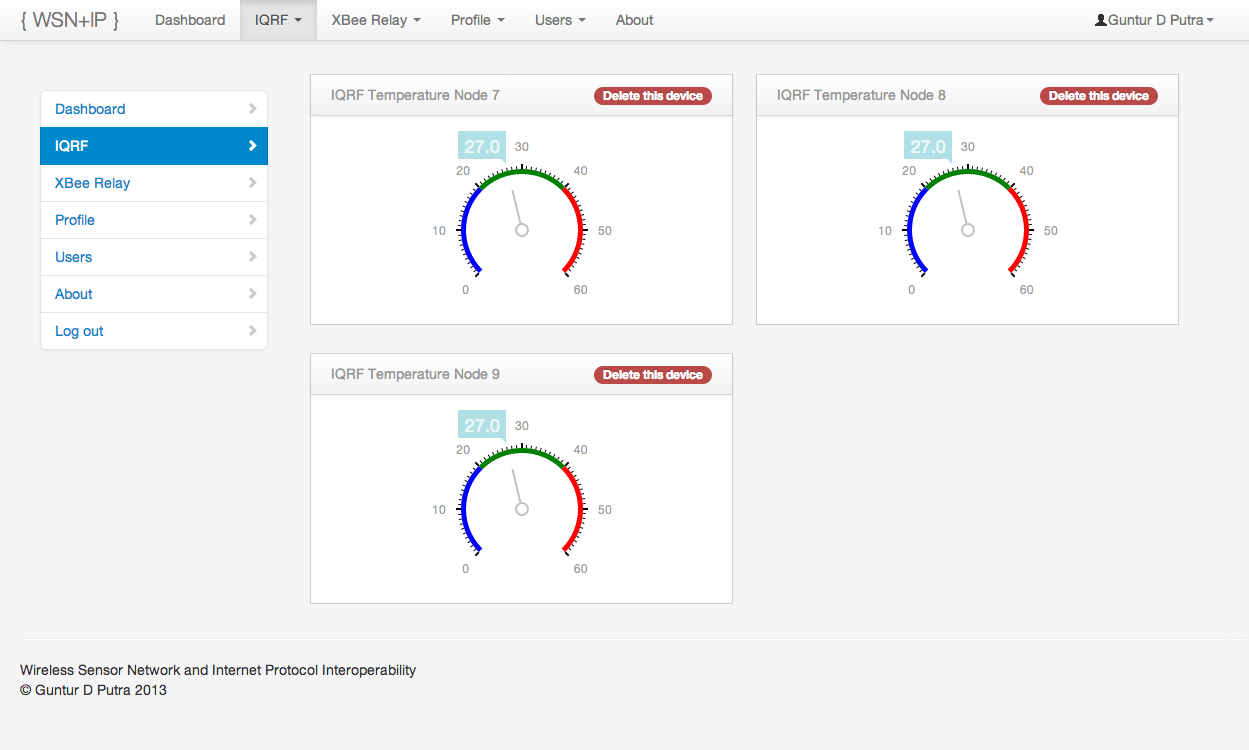
\includegraphics[width=0.9\textwidth]{gambar/iqrf-list}
				    \caption{Halaman daftar piranti IQRF yang terpasang.}
				    \label{iqrf-list}
				\end{figure}

			Pada Gambar \ref{iqrf-list} tertampil tiga buah termometer digital yang masing-masing menampilkan hasil bacaan temperatur dari masing-masing sensor IQRF. Perubahan suhu dapat dilihat secara langsung.

			Pengguna juga dapat melihat semua piranti XBee yang terpasang dengan halaman khusus yang tertera pada Gambar \ref{xbee-list}. Halaman ini akan menampilkan semua piranti XBee yang terdaftar pada aplikasi.

				\begin{figure}[H]
				  \centering
				    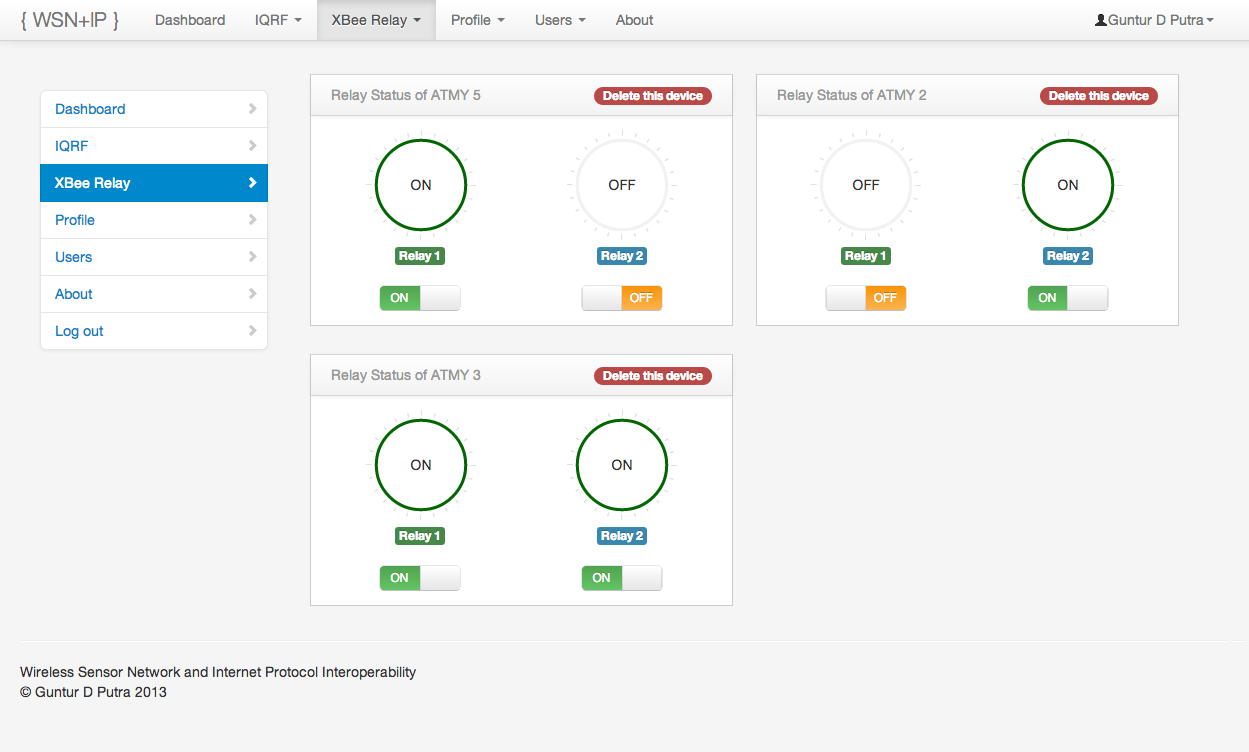
\includegraphics[width=0.9\textwidth]{gambar/xbee-list}
				    \caption{Halaman daftar piranti XBee yang terpasang.}
				    \label{xbee-list}
				\end{figure}

			Seperti yang dapat dilihat pada Gambar \ref{xbee-list}, terdapat tiga piranti XBee yang terdaftar pada aplikasi. Melalui halaman ini, pengguna dapat memati-nyalakan sensor dengan meng-klik saklar yang diinginkan. Dibutuhkan sekitar dua sampai tiga detik untuk menyalakan relay.

			Seperti yang sudah dijelaskan, aplikasi mendukung profil guna otomatisasi tugas-tugas tertentu. Jika pengguna mengiginkan untuk menambahkan profil tertentu, tersedia halaman khusus seperti yang terlihat pada Gambar \ref{profile-add}. Jika suhu yang terbaca di sensor IQRF tertentu mencapai nilai yang diinginkan, maka kondisi relay pada piranti XBee tertentu akan terkonfigurasi seperti yang diinginkan pengguna. Untuk lebih jelasnya bisa dilihat pada Gambar \ref{profile-add}.

				\begin{figure}[H]
				  \centering
				    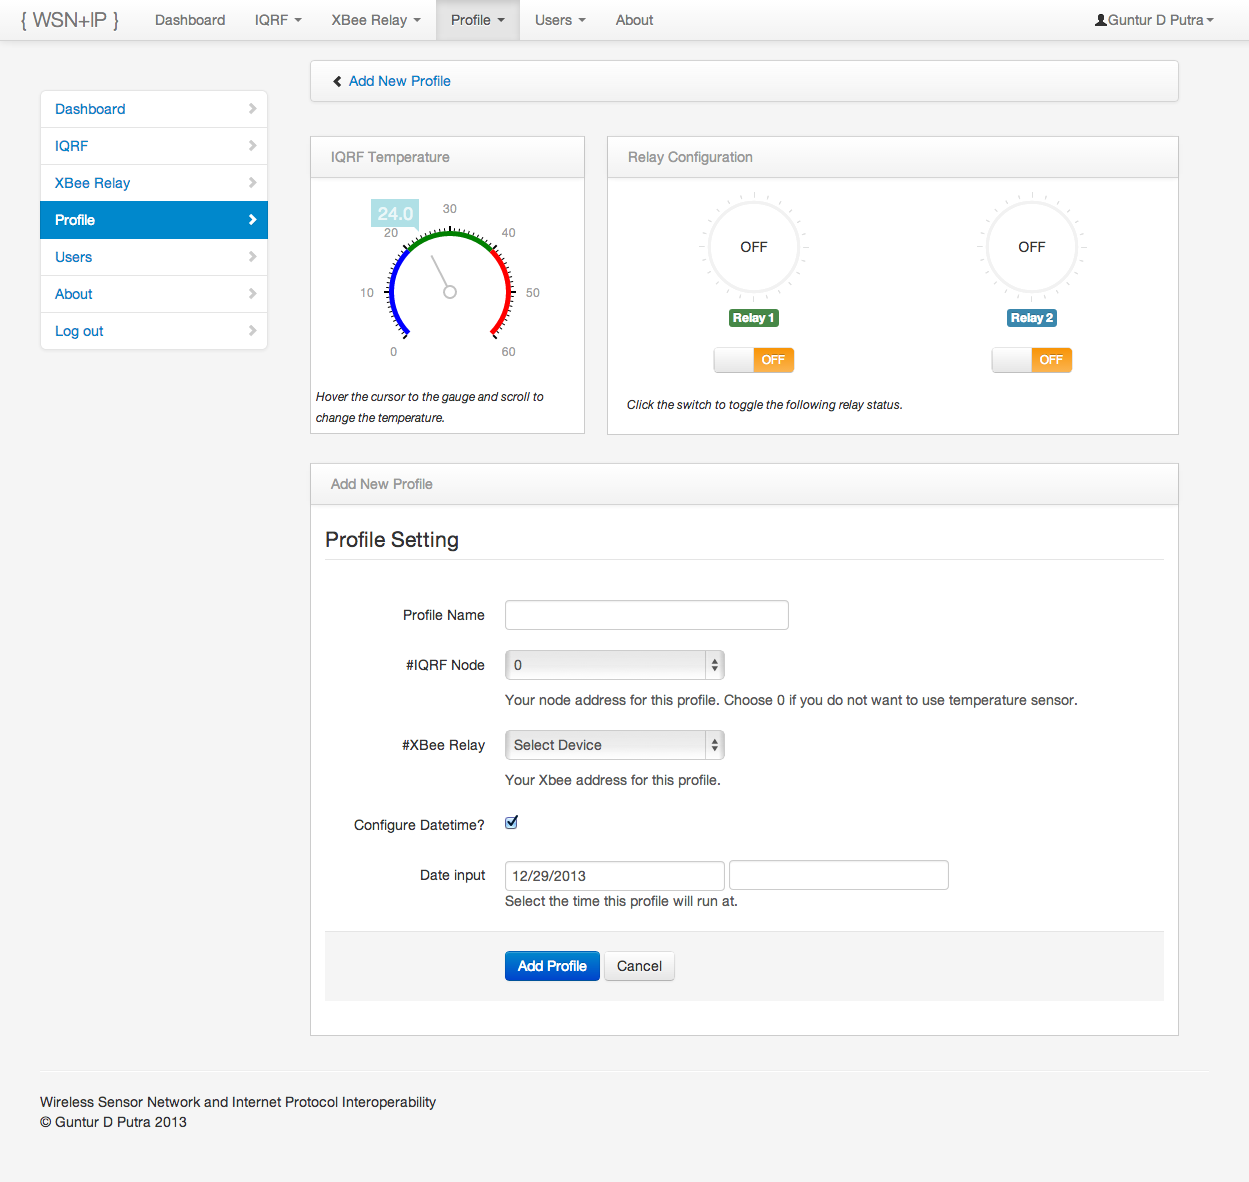
\includegraphics[width=0.9\textwidth]{gambar/profile-add}
				    \caption{Halaman untuk menambahkan profil.}
				    \label{profile-add}
				\end{figure}

			Informasi yang harus dimasukkan ke dalam aplikasi agar pengguna dapat menambahkan profil baru, seperti yang terlihat pada Gambar \ref{profile-add}, adalah:

				\begin{itemize}
					\item temperatur yang diinginkan,
					\item konfigurasi relay saat temperatur tercapai,
					\item nama profil,
					\item alamat sensor IQRF yang diinginkan (pembacaan temperatur),
					\item alamat ATMY piranti XBee yang diinginkan (relay),
					\item dan tanggal dan waktu yang diinginkan.
				\end{itemize}

			Namun jika pengguna hanya ingin menyala-matikan relay XBee pada waktu tertentu, maka pengguna tinggal memilih alamat nol (0) untuk sensor IQRF. Dengan demikian, pembacaan temperatur pada IQRF akan diabaikan.

			Jika pengguna ingin relay XBee terkonfigurasi saat IQRF membaca temperatur tertentu, tanpa memperhatikan tanggal dan waktu, pengguna hanya mencentang \emph{checkbox} yang sudah tersedia. Dengan demikian, profil akan berjalan tanpa memperhatikan waktu tertentu.

			Halaman selanjutnya adalah halaman yang menampilkan semua pengguna yang terdaftar, seperti yang dapat dilihat pada Gambar \ref{user-list}. Namun yang dapat mengakses halaman ini adalah pengguna yang berstatus \emph{administrator}.

				\begin{figure}[H]
				  \centering
				    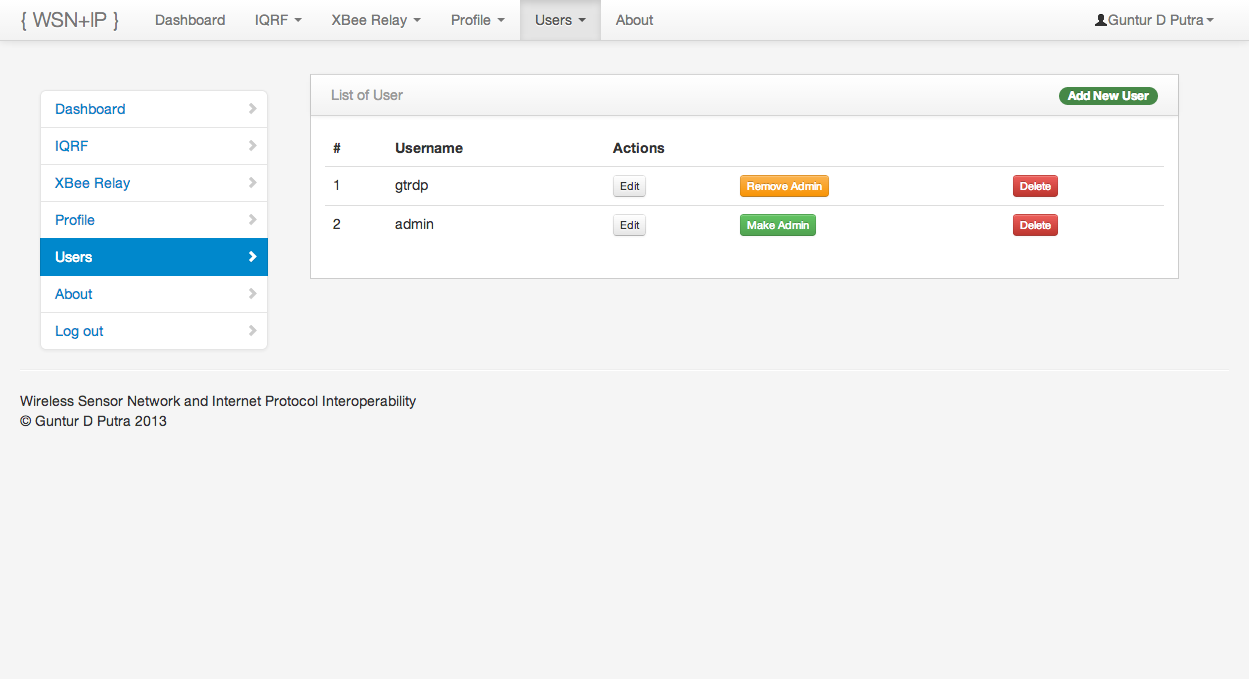
\includegraphics[width=0.9\textwidth]{gambar/user-list}
				    \caption{Halaman yang menampilkan daftar pengguna.}
				    \label{user-list}
				\end{figure}

			Pada halaman ini, terdapat tautan untuk menambahkan pengguna baru, mengedit data pengguna yang sudah terdaftar, menghapus data pengguna, dan menaikkan status pengguna menjadi \emph{administrator} atau menurunkannya.

			Jika pengguna meng-klik tautan untuk menambahkan pengguna baru, maka pengguna akan diarahkan menuju halaman baru seperti yang dapat dilihat pada Gambar \ref{user-add}. Pada halaman ini, pengguna diminta untuk memasukkan informasi-informasi tentang pengguna baru.

				\begin{figure}[H]
				  \centering
				    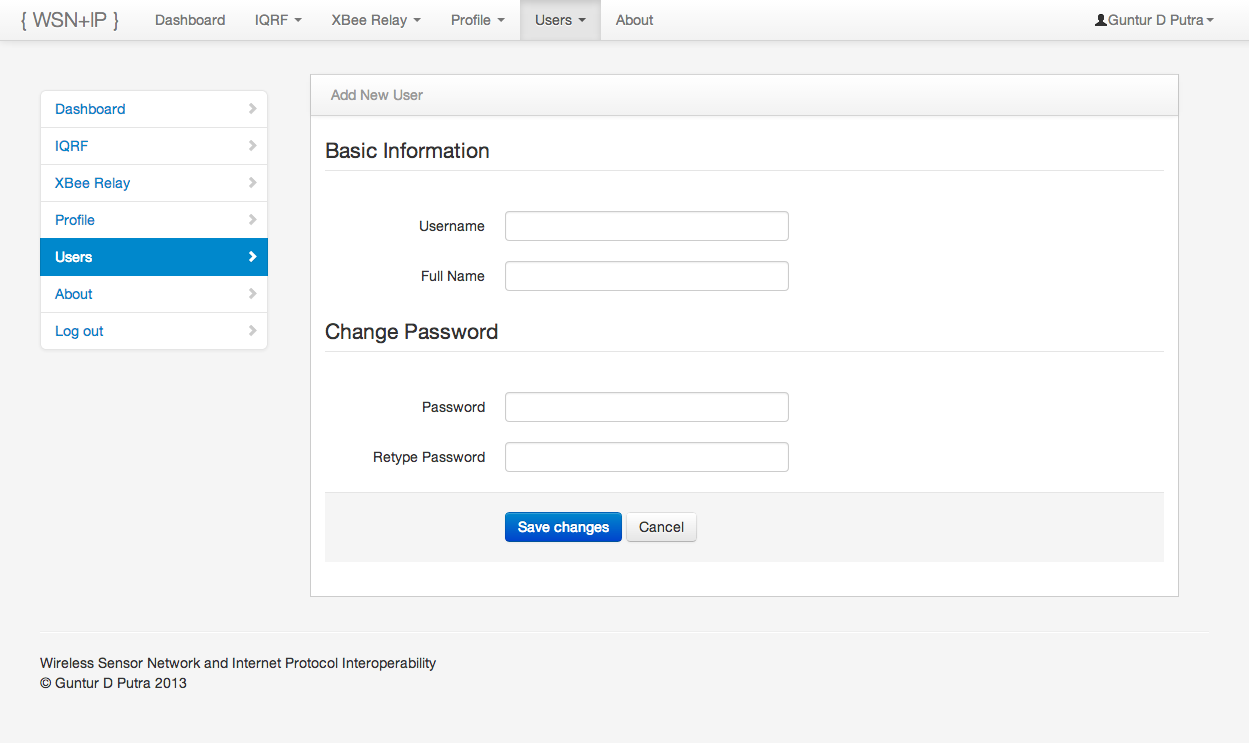
\includegraphics[width=0.9\textwidth]{gambar/user-add}
				    \caption{Halaman untuk menambahkan pengguna baru.}
				    \label{user-add}
				\end{figure}

			Informasi yang harus dimasukkan, seperti yang dapat dilihat pada Gambar \ref{user-add}, antara lain:

				\begin{itemize}
					\item \emph{username} pengguna baru,
					\item nama lengkap pengguna baru,
					\item dan kata sandi pengguna (dua kali).
				\end{itemize}

			Untuk dapat mengakses semua fitur/halaman di atas, pengguna harus \emph{log in} terlebih dahulu. Halaman login dari aplikasi web terlihat pada Gambar \ref{login}.

				\begin{figure}[H]
				  \centering
				    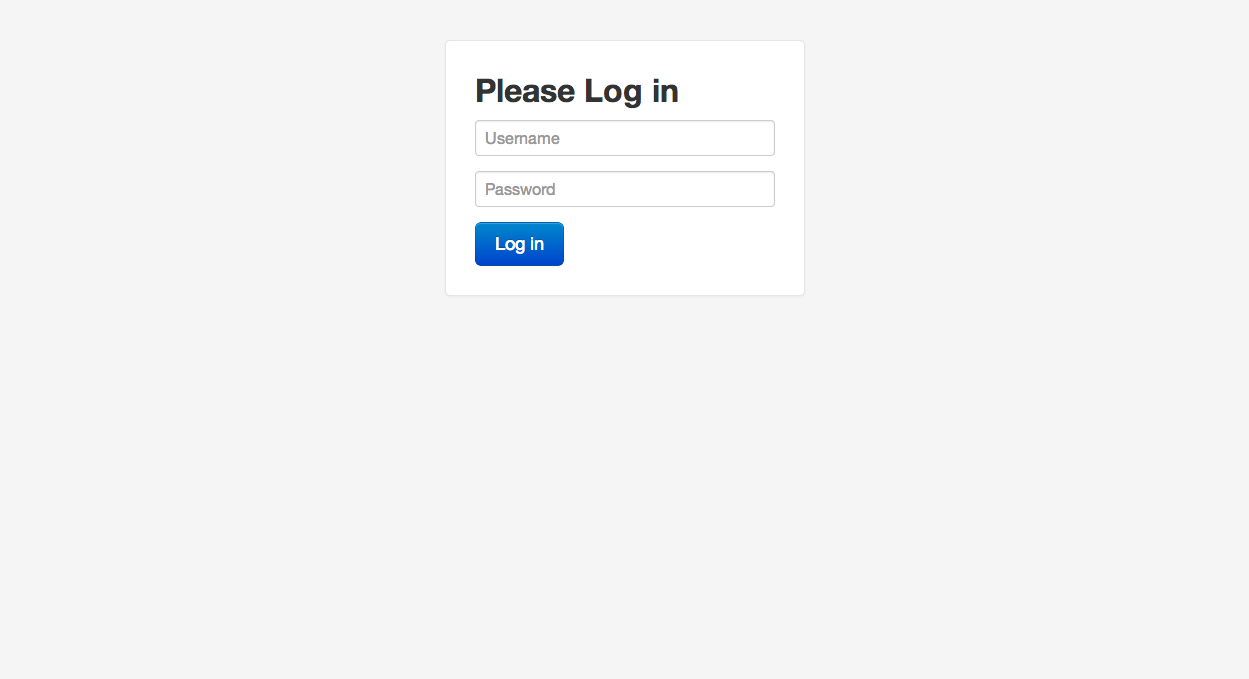
\includegraphics[width=0.9\textwidth]{gambar/login}
				    \caption{Halaman login.}
				    \label{login}
				\end{figure}

			Informasi yang dibutuhkan untuk \emph{log in} hanya \emph{username} atau nama pengguna, dan \emph{password} atau kata sandi.

			Pendekatan yang dilakukan pada aplikasi ini tidak seperti aplikasi web pada umumnya, di mana pengguna dapat mengklik tautan registrasi yang biasanya terdapat pada halaman \emph{log in}. Pendekatan yang dilakukan seperti pada proses \emph{log in} pada komputer. Jadi jika pengguna baru ingin masuk, ia bisa mendaftarkan dirinya melalui pengguna lama yang sudah dapat \emph{log in}, menggunakan halaman yang sudah dijelaskan sebelumnya pada Gambar \ref{user-add}.


		\subsection{Kode Sumber}
			Kode sumber dapat diperoleh pada situs GitHub dengan alamat URL \url{https://github.com/gtrdp/wsn-ip-interoperability}. Pada laman tersebut, kode sumber dapat diunduh dalam format .zip. Dengan bantuan aplikasi git, \emph{project} dari aplikasi ini, lengkap dari aplikasi C, Python, dan Web, dapat di-kloning.


	\section{Analisis Unjuk Kerja Aplikasi}
		Bagian terakhir dari skripsi ini akan ini menjelaskan hal-hal terkait tentang cara perangkaian perangkat keras sehingga dapat difungsikan, instalasi aplikasi ke piranti sehingga sesuai kondisi sesungguhnya, hasil uji coba aplikasi, serta masalah yang dihadapi dan penyelesaiannya.

		\subsection{Instalasi Piranti}
			Perangkat keras pertama yang akan dirakit adalah koordinator IQRF yang tersambung langsung pada AP. Koordinator IQRF ini terdiri atas kabel USB to Serial Prolific, kit pengembangan CK-EVAL-04, dan IQRF TR-52B seperti dapat dilihat pada Gambar \ref{iqrf-coordinator}. Kondisi koordinator sensor IQRF sebelum dirakit dapat dilihat pada Gambar \ref{iqrf-stripped}.

			\begin{figure}[H]
				\begin{subfigure}[b]{\textwidth}
					\centering
				    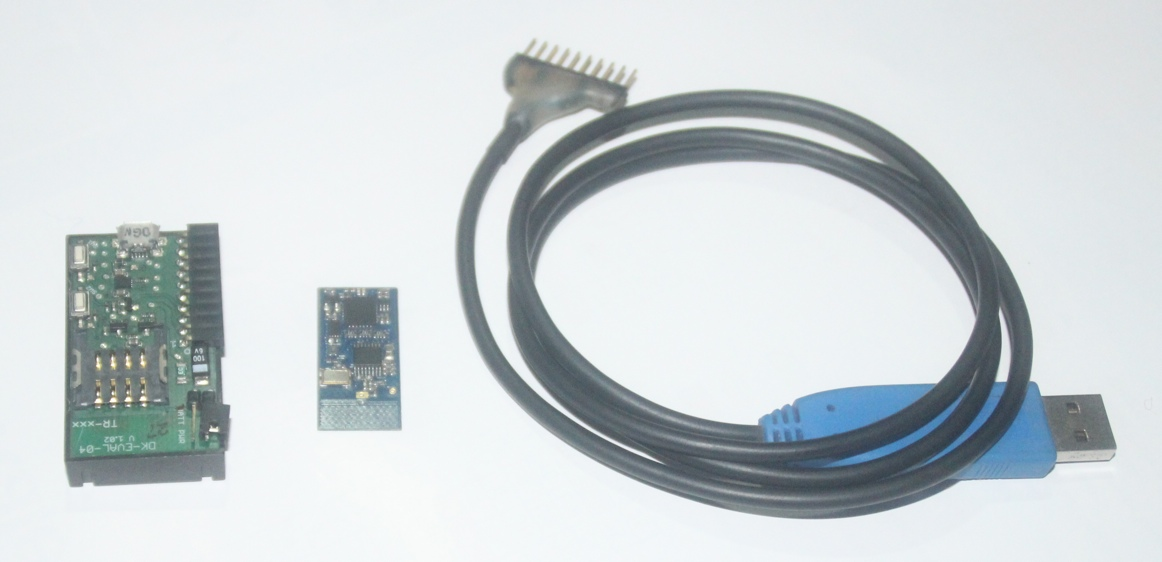
\includegraphics[width=0.7\textwidth]{gambar/iqrf-stripped}
				    \caption{Sebelum dirakit.}
				    \label{iqrf-stripped}
				\end{subfigure}
				 ~
				\begin{subfigure}[b]{\textwidth}
					\centering
				    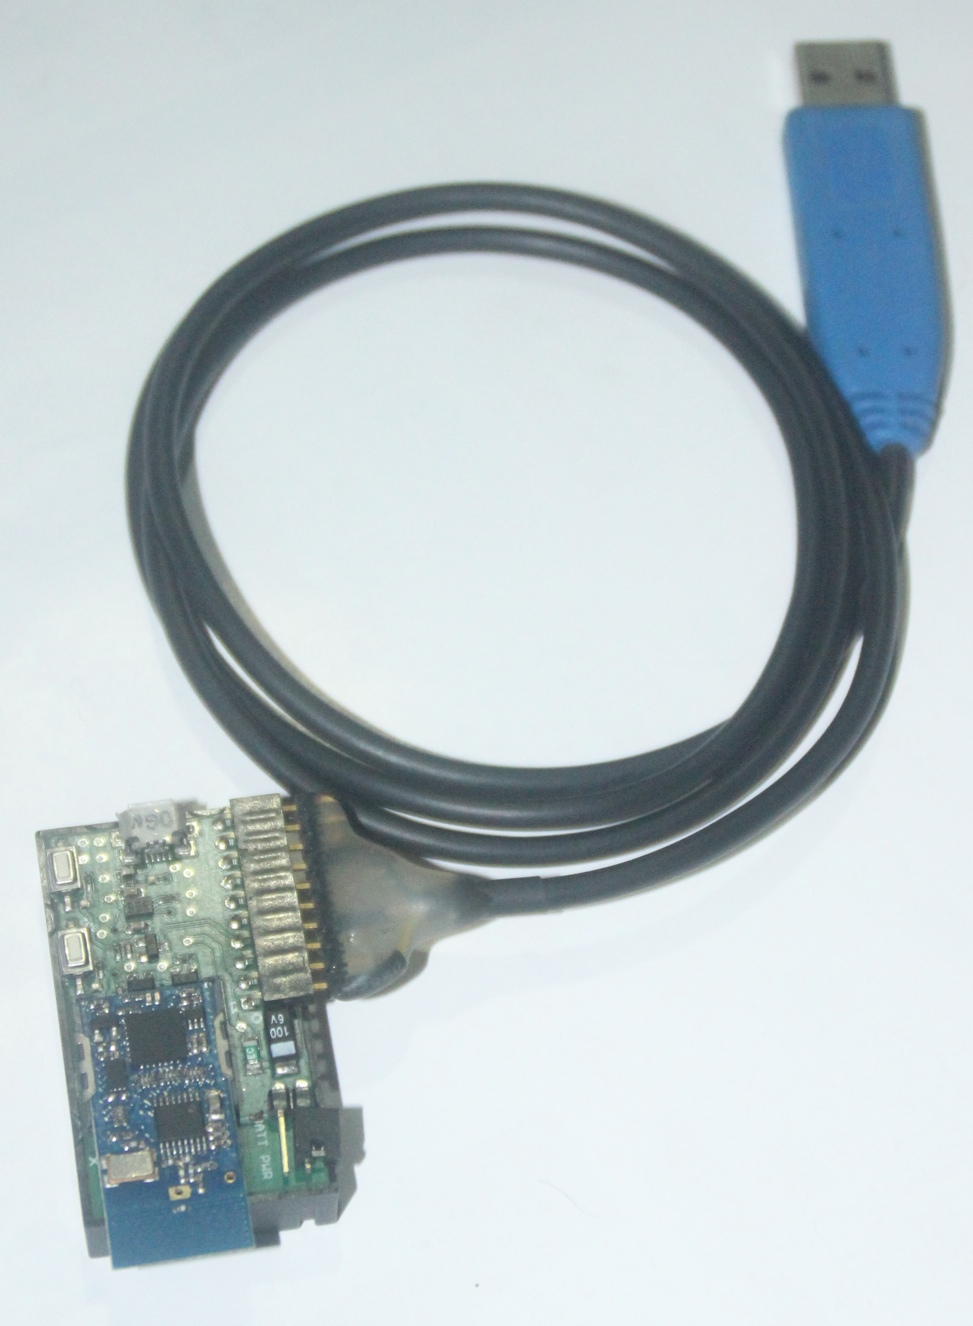
\includegraphics[width=0.5\textwidth]{gambar/iqrf-complete}
				    \caption{Setelah dirakit.}
				    \label{iqrf-complete}
				\end{subfigure}
				\caption{Koordinator sensor IQRF yang akan disambungkan pada AP.}
				\label{iqrf-coordinator}
			\end{figure}

			Kemudian semua bagian disambungkan pada tempatnya. Untuk kabel USB to Serial Prolific, posisi kabel \emph{ground} terpasang pada bagian bawah seperti terlihat pada Gambar \ref{iqrf-complete}.

			Koordinator piranti XBee pada AP terdiri atas \emph{XBee 802.15.4 Radios (Series 1)} dan \emph{XBee Explorer USB Board} yang tersambung pada AP dengan kabel mini-USB seperti dapat dilihat pada Gambar \ref{xbee-sink}.

			\begin{figure}[H]
				\begin{subfigure}[b]{\textwidth}
					\centering
				    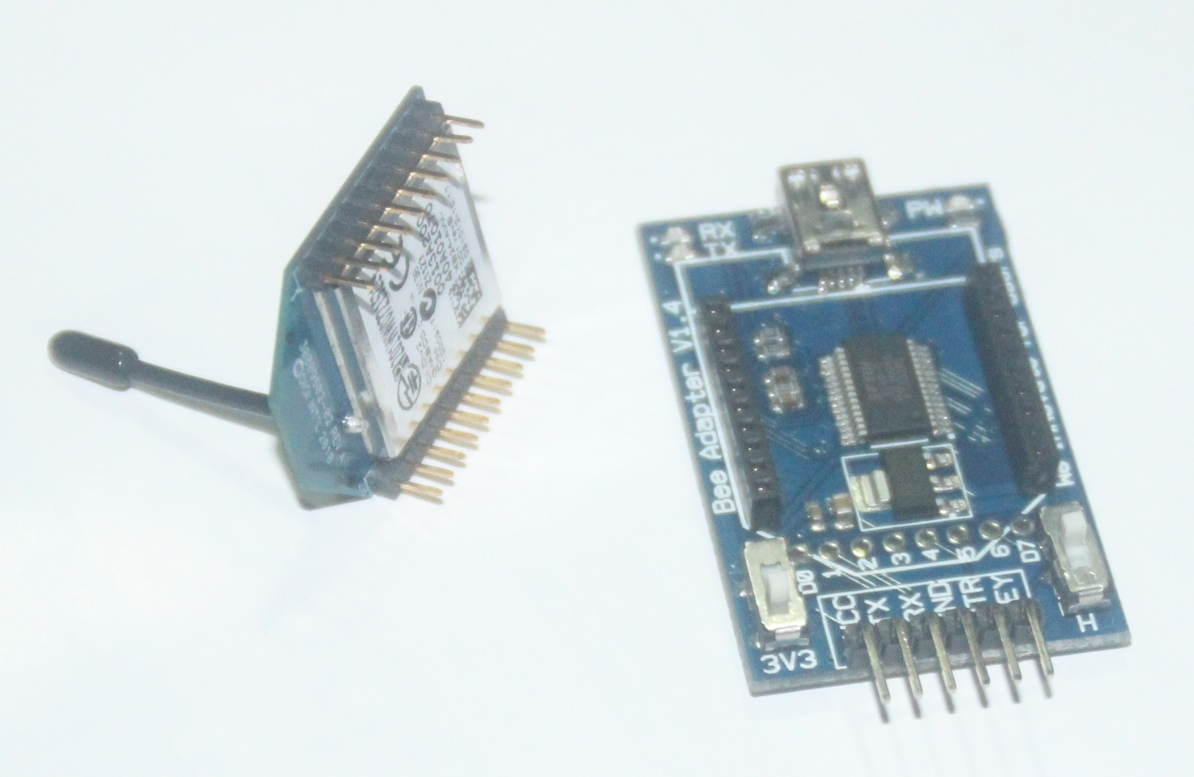
\includegraphics[width=0.5\textwidth]{gambar/xbee-sink-stripped}
				    \caption{Koordinator XBee saat sebelum dirakit.}
				    \label{xbee-sink-stripped}
				\end{subfigure}
				 ~
				\begin{subfigure}[b]{\textwidth}
					\centering
				    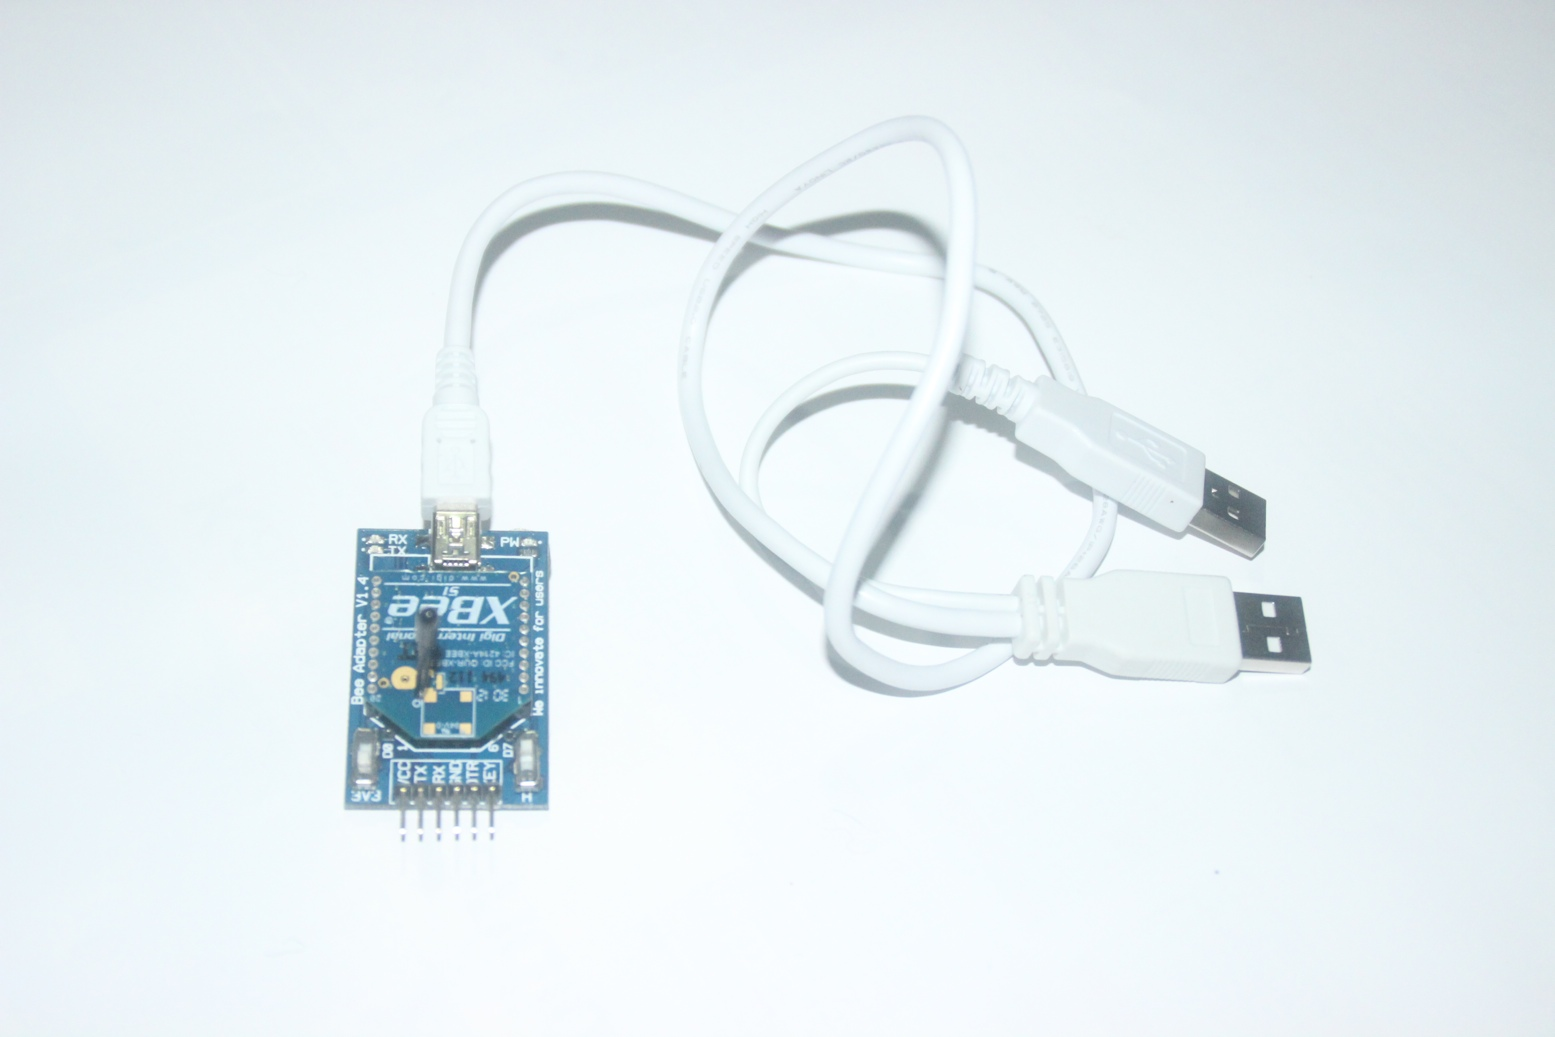
\includegraphics[width=0.7\textwidth]{gambar/xbee-sink-complete}
				    \caption{Koordinator XBee saat telah dirakit.}
				    \label{xbee-sink-complete}
				\end{subfigure}
				\caption{Koordinator piranti XBee yang akan disambungkan pada AP.}
				\label{xbee-sink}
			\end{figure}

			Merakit koordinator piranti XBee termasuk mudah, karena hanya perlu memasang \emph{XBee 802.15.4 Radios (Series 1)} pada \emph{XBee Explorer USB Board}, kemudian menghubungkan keduanya ke AP, seperti yang dapat dilihat pada Gambar \ref{xbee-sink-complete}.

			AP yang digunakan adalah TP-LINK MR3020 dengan USB Hub, seperti yang dapat dilihat pada Gambar \ref{ap-stripped}. USB Hub digunakan untuk menyambungkan USB \emph{flash drive}, koordinator IQRF, dan koordinator XBee.

			\begin{figure}[H]
				\begin{subfigure}[b]{\textwidth}
					\centering
				    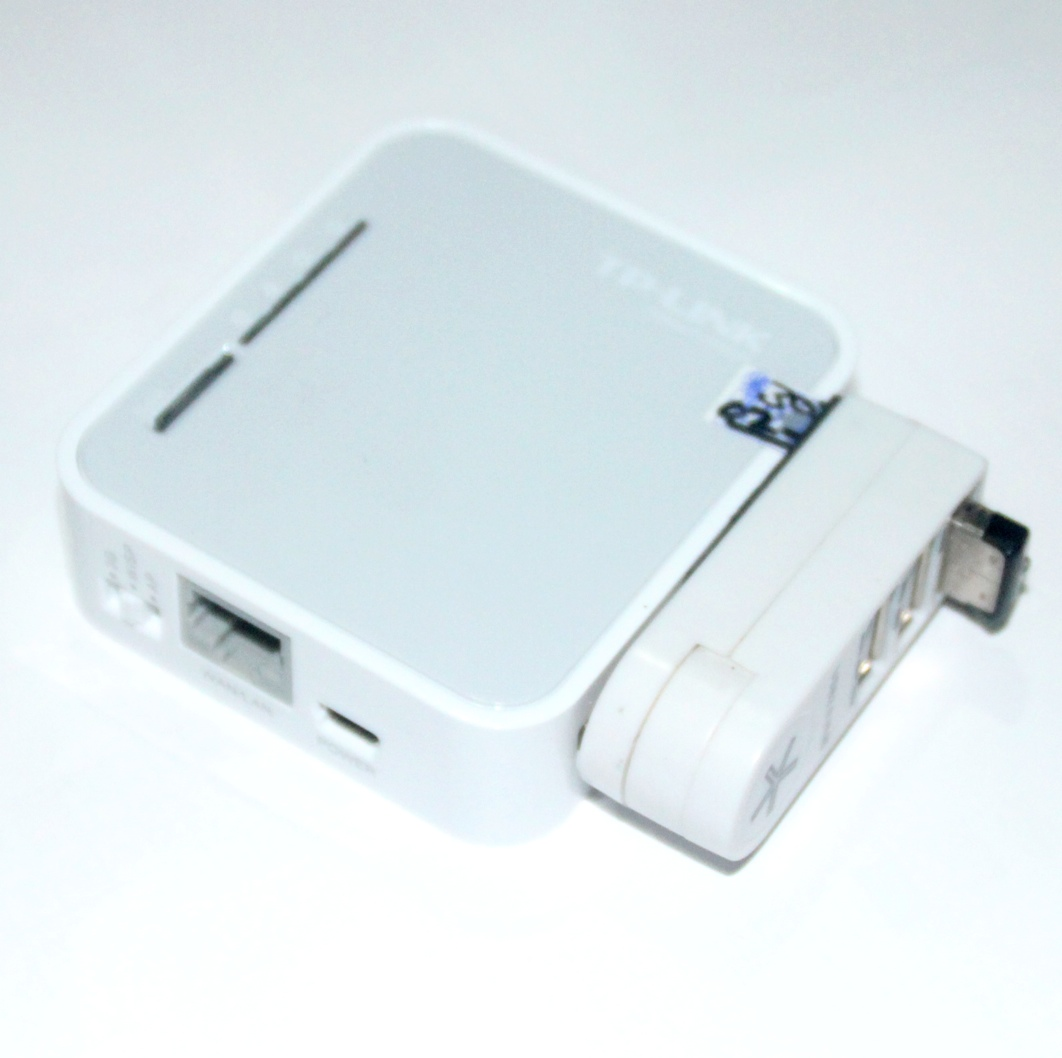
\includegraphics[width=0.5\textwidth]{gambar/ap-stripped}
				    \caption{AP saat sebelum dirakit.}
				    \label{ap-stripped}
				\end{subfigure}
				 ~
				\begin{subfigure}[b]{\textwidth}
					\centering
				    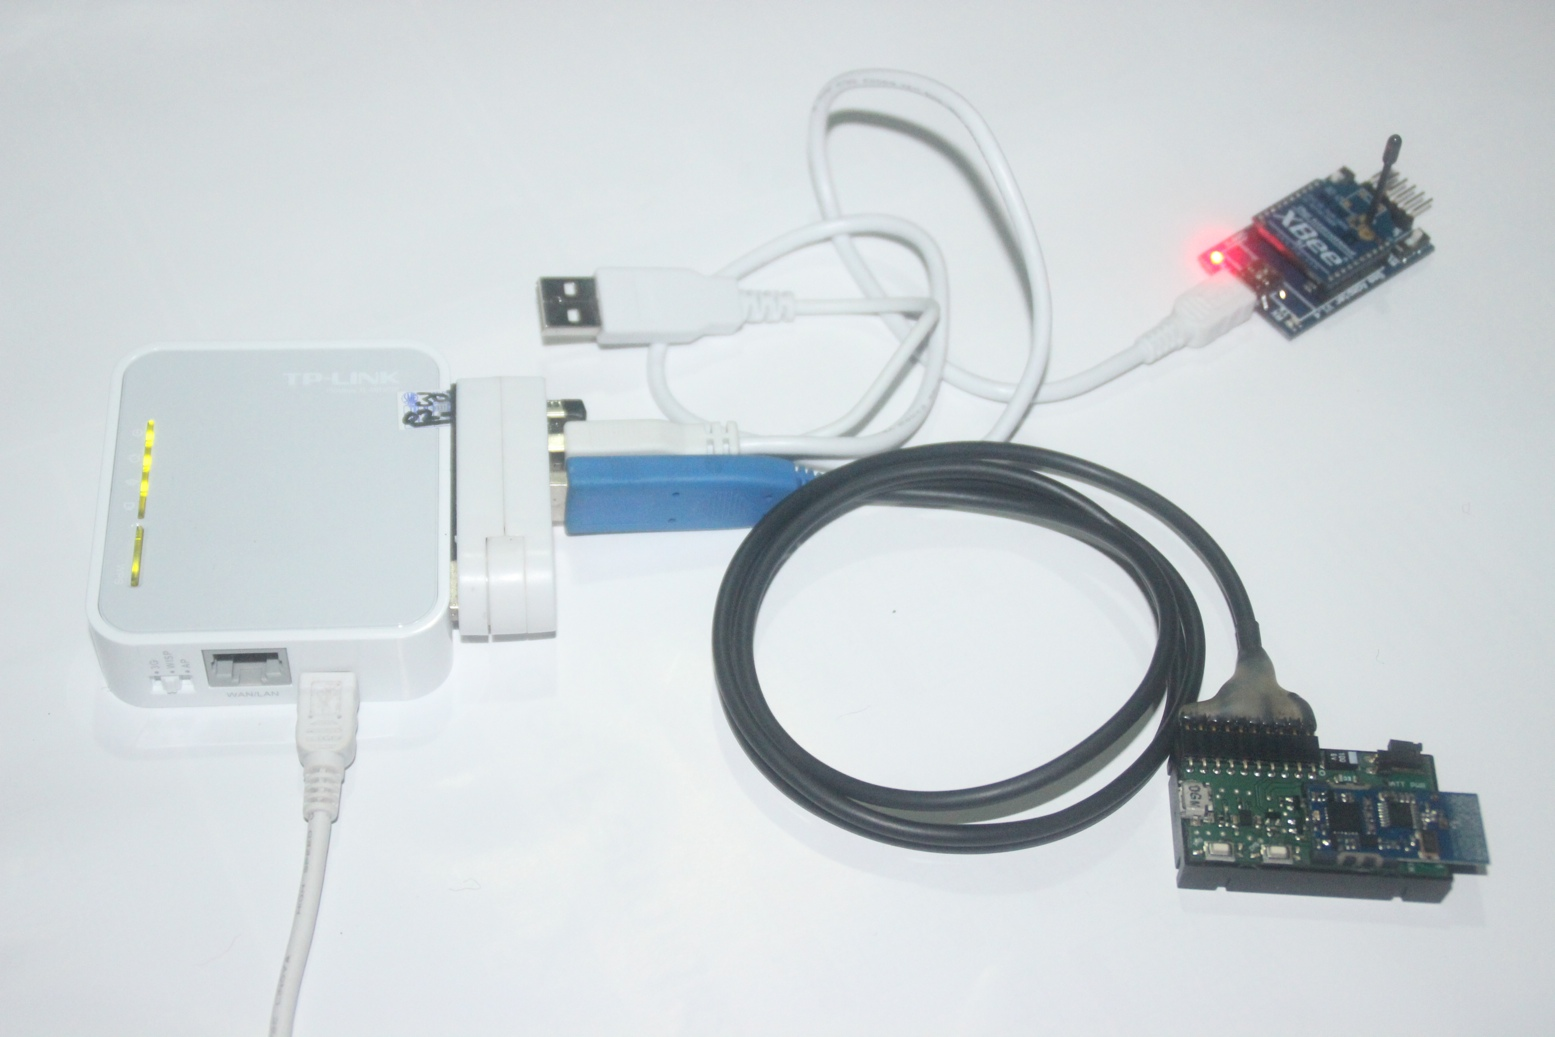
\includegraphics[width=0.7\textwidth]{gambar/ap-complete}
				    \caption{AP saat telah dirakit.}
				    \label{ap-complete}
				\end{subfigure}
				\caption{AP TP-LINK MR3020.}
				\label{ap}
			\end{figure}

			Urutan piranti yang terpasang ke AP, dari atas ke bawah, adalah USB \emph{flash drive}, koordinator XBee, dan koordinator IQRF. Posisi tersebut tidak boleh terbalik karena tidak sesuai dengan konfigurasi aplikasi yang sudah dirancang dan kembangkan. Sehingga kondisi saat semua piranti sudah dipasangkan dapat dilihat pada Gambar \ref{ap-complete}.

			Setelah AP sudah siap, langkah selanjutnya adalah perakitan sensor IQRF dan piranti XBee. Sensor-sensor IQRF terdiri atas TR-52B dan kit pengembangan DK-EVAL-03 seperti dapat dilihat pada Gambar \ref{iqrf-node}.

			\begin{figure}[H]
				\begin{subfigure}[b]{\textwidth}
					\centering
				    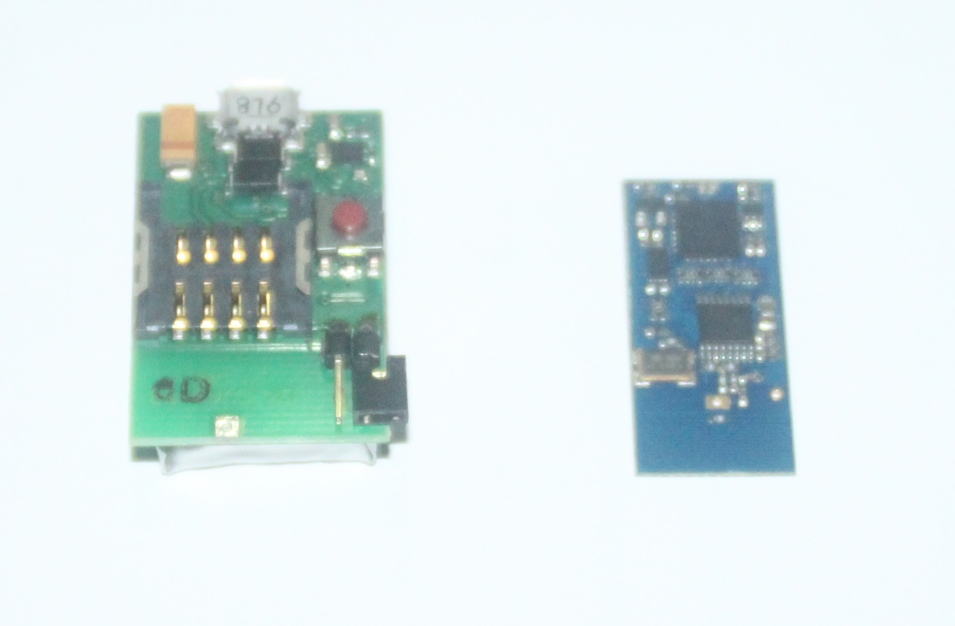
\includegraphics[width=0.4\textwidth]{gambar/iqrf-node-stripped}
				    \caption{Sebelum dirakit.}
				    \label{iqrf-node-stripped}
				\end{subfigure}
				 ~
				\begin{subfigure}[b]{\textwidth}
					\centering
				    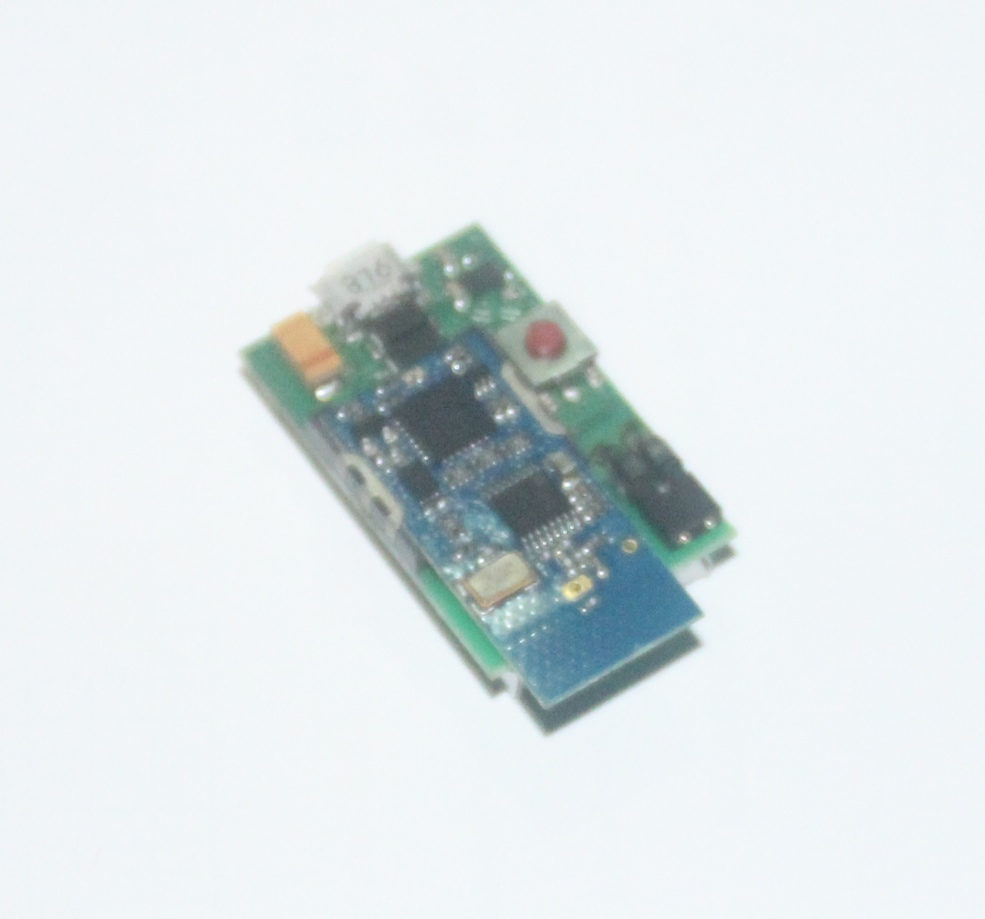
\includegraphics[width=0.4\textwidth]{gambar/iqrf-node-complete}
				    \caption{Setelah dirakit.}
				    \label{iqrf-node-complete}
				\end{subfigure}
				\caption{Sensor IQRF.}
				\label{iqrf-node}
			\end{figure}

			Untuk merakit sensor IQRF, masukkan TR-52B ke dalam kit pengembangan DK-EVAL-03 pada \emph{slot} yang sudah disediakan. Kondisi setelah dipasangkan dapat dilihat pada Gambar \ref{iqrf-node-complete}.

			Sedangkan piranti XBee relay terdiri atas tiga bagian, yaitu \emph{XBee 802.15.4 Radios (Series 1)}, \emph{2 channel Relay Shield For Arduino (With XBee/BTBee interface)}, dan Arduino Uno yang tersambung ke sumber listrik dengan kabel USB seperti dapat dilihat pada Gambar \ref{xbee-relay}.

			\begin{figure}[H]
				\begin{subfigure}[b]{\textwidth}
					\centering
				    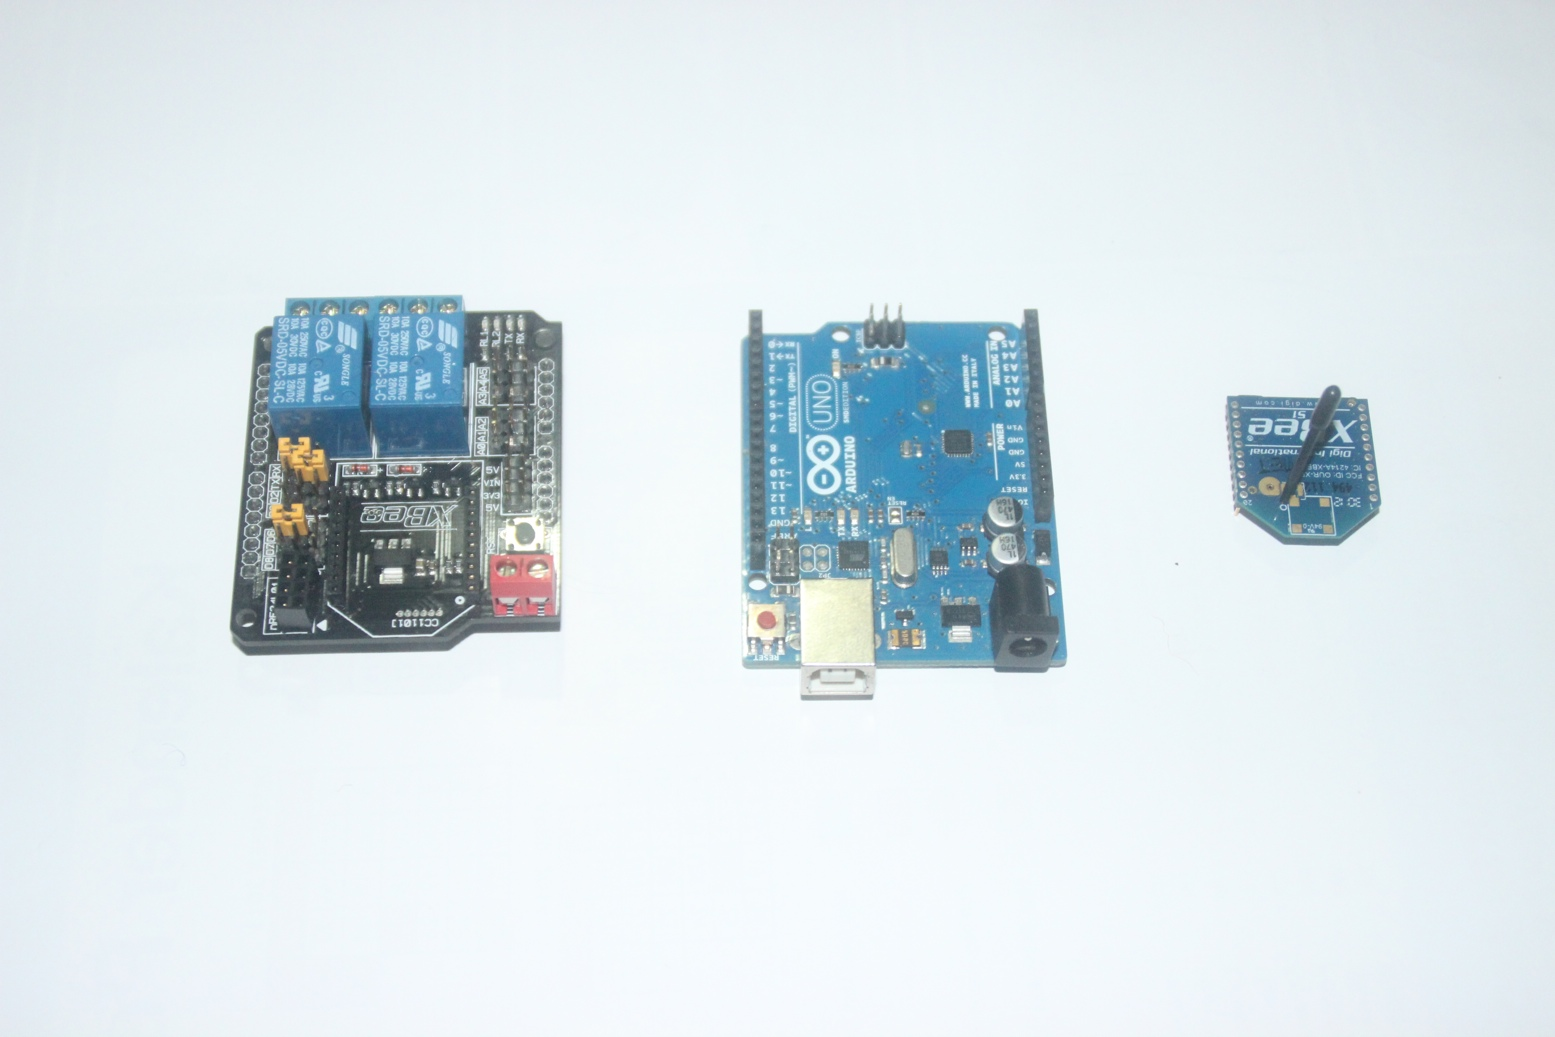
\includegraphics[width=0.7\textwidth]{gambar/xbee-stripped}
				    \caption{Sebelum dirakit.}
				    \label{xbee-stripped}
				\end{subfigure}
				 ~
				\begin{subfigure}[b]{\textwidth}
					\centering
				    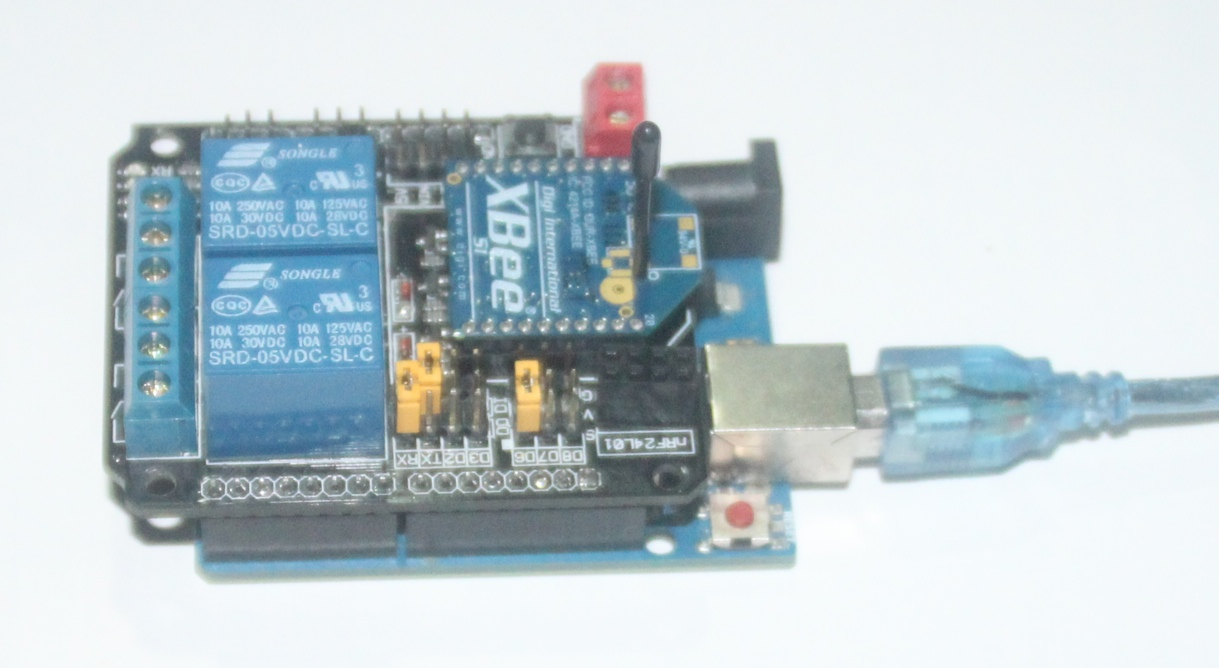
\includegraphics[width=0.7\textwidth]{gambar/xbee-complete}
				    \caption{Setelah dirakit.}
				    \label{xbee-complete}
				\end{subfigure}
				\caption{Piranti XBee.}
				\label{xbee-relay}
			\end{figure}

			Piranti XBee akan tersusun dalam tiga lapis rangkaian, mulai dari bawah, Arduino Uno, \emph{2 channel Relay Shield For Arduino (With XBee/BTBee interface)}, dan \emph{XBee 802.15.4 Radios (Series 1)}. Hasil rakitan piranti XBee dapat dilihat pada Gambar \ref{xbee-complete}.

		\subsection{Hasil Uji Coba Aplikasi}
			Uji coba yang dilakukan menggunakan satu set AP lengkap yang sudah dilengkapi dengan koordinator IQRF dan XBee. Sensor yang digunakan adalah dua buah IQRF dan satu buah XBee.

			Uji coba pertama dilakukan dengan penambahan XBee Relay baru via aplikasi web dan menyalakan relay 1 dengan ponsel cerdas seperti dapat dilihat pada Gambar \ref{xbee-action}. Pada Gambar \ref{xbee-action} dapat dilihat bahwa relay 1 dalam keadaan menyala pada layar ponsel cerdas dan XBee Relay.

			\begin{figure}[H]
			  \centering
			    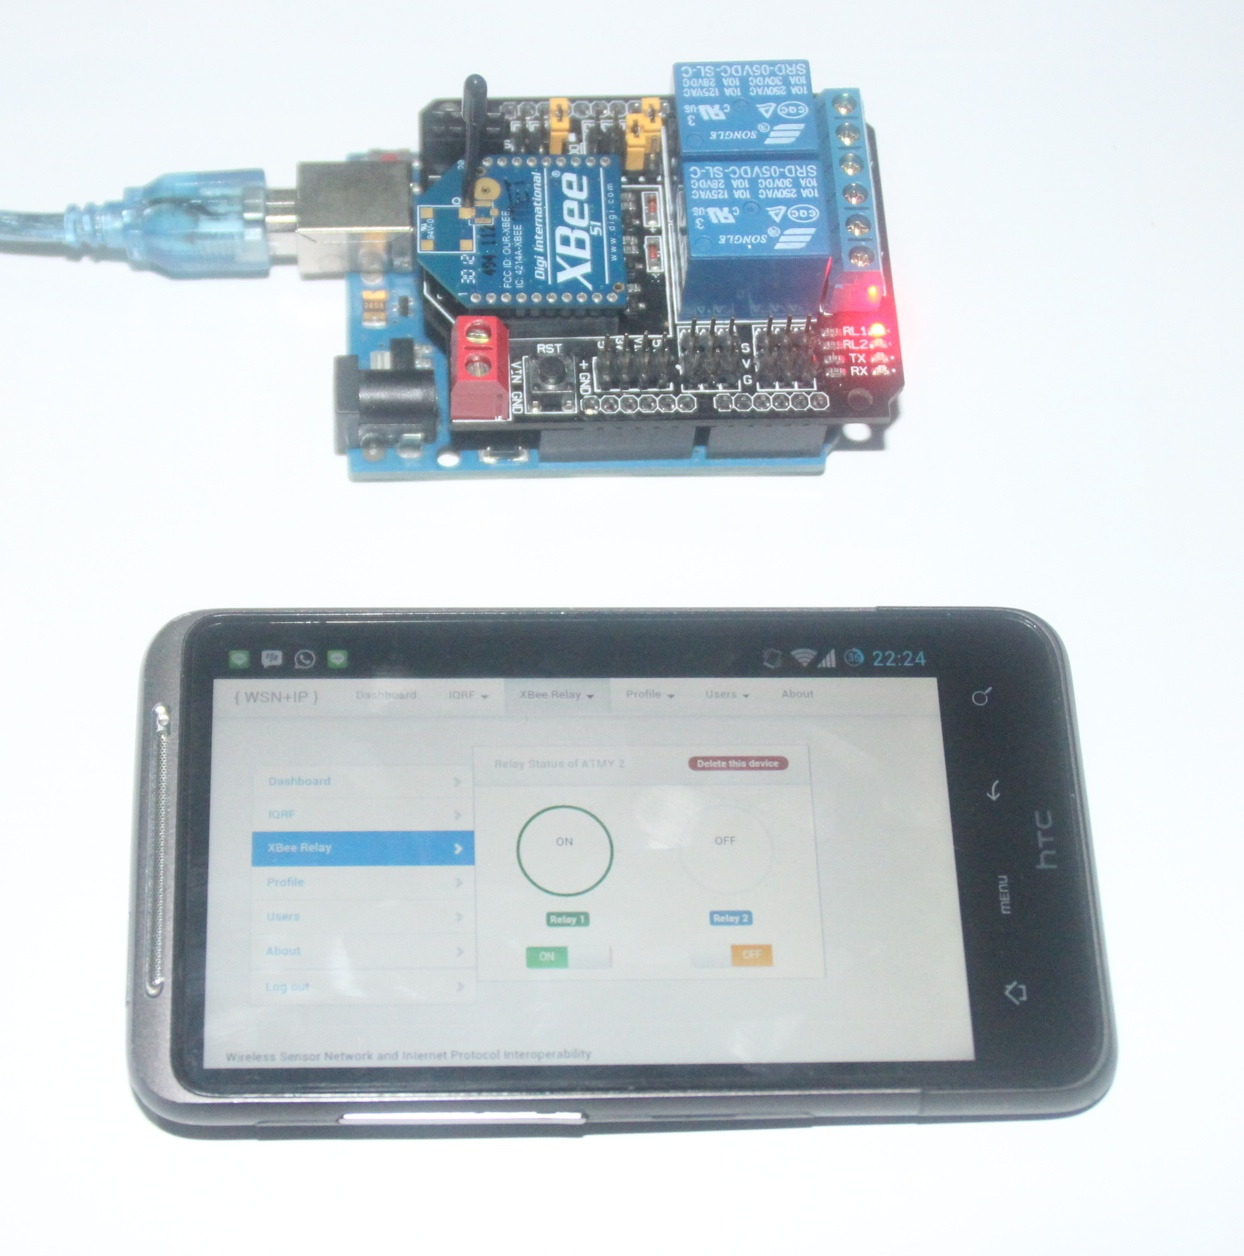
\includegraphics[width=0.7\textwidth]{gambar/xbee-action}
			    \caption{Uji coba aplikasi dengan ponsel cerdas.}
			    \label{xbee-action}
			\end{figure}

			Pada saat pengguna meng-klik salah satu saklar, akan tampak \emph{progress} dari proses menyalakan relay berupa garis tepi lingkaran berwarna hijau. Saat relay sudah dalam kondisi menyala, maka lingkaran akan mempunyai garis tepi berwarna hijau yang sempurna.

			Pengujian IQRF dilakukan dengan penambahan dua sensor via aplikasi web dan kemudian melihat temperatur yang terbaca. Salah satu sensor digenggam dengan tangan untuk memanipulasi temperatur. Hasilnya dapat dilihat pada Gambar \ref{screenshot-iqrf}.
			
			\begin{figure}[H]
			  \centering
			    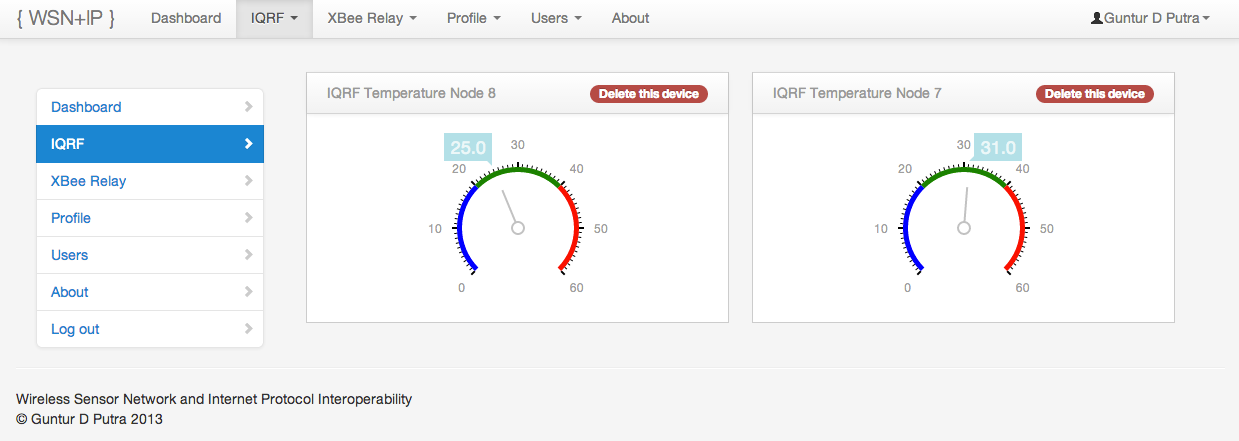
\includegraphics[width=0.9\textwidth]{gambar/screenshot-iqrf}
			    \caption{Membaca temperatur yang terbaca pada sensor.}
			    \label{screenshot-iqrf}
			\end{figure}

			Jarum penunjuk pada masing-masing penampil akan bergerak sesuai dengan bacaan temperatur dari masing-masing sensor IQRF. Gerakan akan terjadi secara langsung, tanpa pengguna harus memuat ulang halaman web.

			Pengujian yang dilakukan pada penelitian ini tidak ditujukan pada ketelitian pembacaan temperatur pada sensor IQRF karena penelitian ini hanya berfokus pada fungsionalitas sistem.
			
			Dari hasil pengujian di atas, didapati bahwa aplikasi yang dibangun sudah dapat berfungsi sebagaimana mestinya.

		\subsection{Kelebihan dan Kekurangan Sistem}
			Secara garis besar, sistem yang dibangun mampu menginteroperabilitaskan dua jenis jaringan sensor nirkabel dan protokol internet dengan biaya yang rendah. Untuk lebih jelasnya, kelebihan sistem yang dibangun dijelaskan pada daftar berikut,

			\vspace{-0.5cm}
			\begin{itemize}
			\begin{singlespace}
				\item mampu mengintegerasikan dua jenis WSN,
				\item jumlah piranti yang terpasang dapat ditambah dan dikurangi secara mudah,
				\item aplikasi web yang dibangun dapat diakses dari komputer maupun ponsel cerdas karena bersifat responsif,
				\item mendukung fitur profil guna mendukung implementasinya pada \emph{green building} dan \emph{smart house},
				\item biaya yang dibutuhkan tergolong murah, dan
				\item AP berukuran kecil sehingga mudah ditempatkan di sudut ruangan.
			\end{singlespace}
			\end{itemize}

			Sedangkan kekurangan sistem yang dapat dikembangkan atau diperbaiki pada penelitian selanjutnya dijelaskan pada daftar berikut ini,

			\vspace{-0.5cm}
			\begin{itemize}
			\begin{singlespace}
				\item skalabilitas yang kurang karena hanya mampu mendukung dua jenis WSN secara \emph{default},
				\item baterai IQRF \emph{node} harus diisi ulang dalam waktu berkala,
				\item memori eksternal dari AP kurang stabil, baru terbaca setelah AP dinyalakan ulang, dan
				\item sistem tidak memiliki baterai cadangan apabila listrik mati.
			\end{singlespace}
			\end{itemize}

		\subsection{Masalah dan Penyelesaian}
			Masalah yang pertamakali muncul adalah tentang extroot. TP-LINK MR3020 memiliki \emph{bug} yang membuat memori eksternal tidak berfungsi saat \emph{booting} pertamakali. Setelah TP-LINK MR3020 dijalankan ulang, memori eksternal baru terbaca. Penyebab dari masalah ini belum ditemukan, sehingga solusi untuk masalah ini adalah melakukan \emph{rebooting} jika TP-LINK MR3020 tidak membaca memori eksternal. Masalah ini tidak ditemukan pada AP dengan jenis lain seperti pada penelitian yang dilakukan oleh \cite{wibowo2013wireless}.

		%	Komunikasi serial yang kata perkata.
			
			IQRF dinilai kurang stabil, terlebih saat menancapkan kabel USB to Serial Prolific ke USB Hub pada AP saat AP sudah menyala. Jika kurang berhati-hati, AP justru akan menjadi tidak stabil. Gejala yang muncul seperti pustaka PHP yang tidak terbaca, sampai jaringan Wi-Fi yang terputus. Untuk mengantisipasi masalah ini, sebaiknya semua kabel terpasang sebelum AP dinyalakan.
			
% Baris ini digunakan untuk membantu dalam melakukan sitasi.
% Karena diapit dengan comment, maka baris ini akan diabaikan
% oleh compiler LaTeX.
\begin{comment}
\bibliography{daftar-pustaka}
\end{comment}